\documentclass[11pt]{article}

\usepackage[margin=1in]{geometry}
\usepackage[T1]{fontenc}
\usepackage[utf8]{inputenc}
\usepackage{lmodern}
\usepackage{microtype}
\usepackage{amsmath,amssymb}
\usepackage{amsthm}
\newtheorem{proposition}{Proposition}
\usepackage{booktabs}
\usepackage{array}
\usepackage{graphicx}
\usepackage{framed}
\usepackage{algorithm}
\usepackage{algpseudocode}
\usepackage{authblk}
\usepackage[numbers]{natbib}
\usepackage[colorlinks=true,linkcolor=blue,citecolor=blue,urlcolor=blue]{hyperref}

\title{One GEMM, Many Subgames: A Predictive Cost Model and an End-to-End
Wall-Clock Win for Iterated Resolving in Imperfect-Information Games}

\author{Max Zhang}
\affil{Independent Researcher}
\date{June 10, 2026}

\begin{document}

\maketitle

\begin{abstract}
Depth-limited search with learned value functions in imperfect-information games
repeatedly solves many public-belief subgames. This work isolates a systems lever in
that loop: at a fixed public cut, resolving generates same-topology subgames that differ
only in entry beliefs and solver state. \textbf{Population fusion} compiles that shared
topology once into a level-grouped structure-of-arrays and runs each finite-iteration
CFR+ update across the whole population as batched tensor operations. The formal timing
model is a floor/slope model,
$C_{\rm seq}(N)=a_s+b_s(N-1)$ and
$C_{\rm fus}(N)=a_f+b_f(N-1)$; the familiar
$\min(N,1/\varphi)$ expression is the launch-bound envelope, not a universal plateau
predictor. On launch-bound Goofspiel-4, the tool-symmetric \texttt{torch.compile}
comparison gives 11.36$\times$ inner and 7.38$\times$ total-wall speedup over 5 matched
CUDA seeds, against a 7.39$\times$ Amdahl ceiling and with no gross divergence under the
paper's predeclared descriptive band check. The eager-dispatch isolate gives
11.79$\times$ inner and 9.99$\times$ total-wall speedup. On saturated Goofspiel-5, a
quiet-host paired run gives 2.40$\times$ inner and 2.00$\times$ total timing speedup;
this is saturated-regime timing-transfer evidence, with the full statistical CUDA
non-divergence run still pending. The contribution is validated population-level
cost-per-solve amortization for iterated resolving, not lower exploitability or
poker-bot strength.
\end{abstract}

\section{Introduction}

Sound depth-limited search with learned value functions is a major template for
two-player zero-sum imperfect-information games. DeepStack~\citep{Moravcik2017} uses
continual re-solving with learned counterfactual values; ReBeL~\citep{Brown2020} brings
public-belief search into reinforcement learning and decision-time play; Student of
Games~\citep{Schmid2023} unifies search-based agents across perfect- and
imperfect-information games. The train-time target-generation loop studied here is the
iterated-resolving pattern in this lineage: repeatedly re-solve small depth-limited
lookahead games (``subgames'') to generate value-network training targets. The depth
limit is what makes each solve affordable, but it cannot be naive: in an
imperfect-information game the value of a position depends on what both players
\emph{believe} about the hidden information, so a search leaf must be valued
conditional on those beliefs --- the public state together with the two players' belief
distributions is the \emph{public belief state} (PBS) --- and truncating the lookahead
without belief-conditioned leaf values yields exploitable
strategies~\citep{BrownSandholm2018}. The inner solver throughout is
CFR+~\citep{Tammelin2014,Tammelin2015,Bowling2015}, an iterative no-regret algorithm
whose time-averaged strategy converges to a Nash equilibrium (primer in \S2.1),
descended from CFR~\citep{Zinkevich2007}. The wall-clock cost of the resolving phase
factors as
\begin{equation}
C \;=\; \underbrace{N_{\text{solves}}}_{\text{how many subgames}} \;\times\;
\underbrace{T}_{\text{CFR iterations per solve}} \;\times\;
\underbrace{c_{\text{solve}}}_{\text{wall-clock per solve-iteration}} ,
\label{eq:cost}
\end{equation}
an accounting identity in which $N_{\text{solves}}$ counts subgame solves over the run,
$T$ is the per-solve CFR+ iteration budget, and $c_{\text{solve}}$ is the average
wall-clock per solve-iteration (the loop's remaining phases --- network training,
measurement --- sit outside it and are handled by the Amdahl analysis of \S6.2). The
inner re-solve dominates the loop: in our instrumented training runs it accounts for
98.4\% of baseline loop wall-clock at our Goofspiel-4 (G4) operating point (\S3).

\textbf{One factor of Eq.~(\ref{eq:cost}) is under-isolated.} Prior work actively
attacks the number of solves, the iterations each solve needs, the variance of sampled
traversals, and the size of each subgame (\S3 compresses the taxonomy; \S7 gives it in
full). The cost per solve-iteration, $c_{\text{solve}}$, has been attacked only
\emph{within} a single tree, by parallelizing one solve's tree walk on the
GPU~\citep{Kim2024,KimSandholm2026}. Amortizing $c_{\text{solve}}$ \emph{across the
population of subgames that one resolving sweep generates} is, to our knowledge, not
isolated and validated as an end-to-end population-level lever in published work (the
related-work delimitation and the structural distinctions from the nearest neighbors
are in \S7).

\textbf{The structural observation, and the mechanism.} Iterated resolving does not
produce one subgame at a time; it produces a \emph{population}. At a fixed depth cut,
every public outcome on the cut frontier roots its own depth-limited subgame, and within
a game these continuation trees share their topology: they differ only in the data
flowing through them --- each player's entry beliefs, or \emph{ranges} (a range is a
probability vector over a player's possible private states), and per-subgame solver
state. Many same-shaped small problems differing only in data is exactly the workload
that batched BLAS~\citep{Abdelfattah2016} and FlashAttention-style kernel
engineering~\citep{Dao2022} --- whose mechanism + cost-model + end-to-end-win template
this paper follows --- taught the systems community to exploit: fuse them, so the device
does the same arithmetic under far fewer kernel launches. We call the resulting
mechanism \textbf{population fusion}: compile the shared topology once into a
level-grouped structure-of-arrays (SoA), and execute each CFR+ iteration of \emph{all}
subgames as one fixed sequence of batched tensor ops (Figure~\ref{fig:hero}; \S4). The
``GEMM'' in the title names this systems pattern --- many same-shaped small solves
turned into one batched tensor workload --- not literal matrix multiplication at every
step. The
fusion axis is $K$, the number of distinct public outcomes at the cut; the
within-outcome private-hand dimension is classical range-vector CFR and is present in
both of our timing arms (\S2.2). The fused solver is verified to match the per-tree
finite-iteration CFR+ outputs under the gates of \S4.5.

\textbf{A predictive cost model.} When does fusion pay? A controlled sweep gives a
floor/slope answer,
$C_{\rm seq}(N)=a_s+b_s(N-1)$ and
$C_{\rm fus}(N)=a_f+b_f(N-1)$: speedup is near-linear when the fused marginal slope is
near zero, and contracts to a slope ratio once one subgame already fills the device
(\S6.1). The simplified $\min(N,1/\varphi)$ form is useful as the launch-bound envelope
and regime intuition, while a two-point marginal-cost probe classifies which
regime a workload is in before committing to fusion.

\textbf{The win survives a real training loop.} Microbenchmark speedups routinely
evaporate inside end-to-end systems; this one does not, because the loop is dominated by
exactly the phase we fused. On Goofspiel-4 --- small subgames, the launch-bound regime
--- the fused inner re-solve is 11.79$\times$ faster than the same kernel applied
per-tree, against the 11.7$\times$ the microbenchmark sweep predicted ex ante, and total
training wall-clock improves 9.99$\times$ against the 10.09$\times$ Amdahl ceiling
implied by the measured inner fraction (5 matched seeds; derivation in \S6.2). The
speedup buys no lower-exploitability claim: the arms pass the paper's broad descriptive
band check --- fused median 0.0402, sequential 0.0469, where for scale uniform random play
scores $\approx$1.42 on this game and 0 is exact Nash. On Goofspiel-5, where a single
subgame already fills the device, the loop realizes the predicted saturated speedups:
2.40$\times$ inner and 2.00$\times$ total (3 matched seeds; \S6.4). As a directional
calibration only, a search-free NFSP baseline trained on the same game remains near
uniform after 600 s --- a budget roughly eight times the fused loop's entire run
(\S6.3).

\textbf{Scope.} The G4 training claims are \emph{equal-band-faster} --- the same broad
descriptive final-exploitability band in less wall-clock --- never lower exploitability,
and never strength against poker bots. The G5 paired run is a saturated-regime
timing-transfer result with CPU/single-solve parity; the full statistical CUDA non-divergence run
remains future work. The headline eager comparisons are same-substrate, against the same
kernel run per-tree; the measured launch-amortization ablation and the G4
compile-vs-compile end-to-end check show that the advantage survives tool symmetry
(\S4.6, \S6.5). The demonstrated loop is a 2-level, single-cut instance, on one game
family and one device; \S8 states every limitation in full.

\begin{figure}[t]
\centering
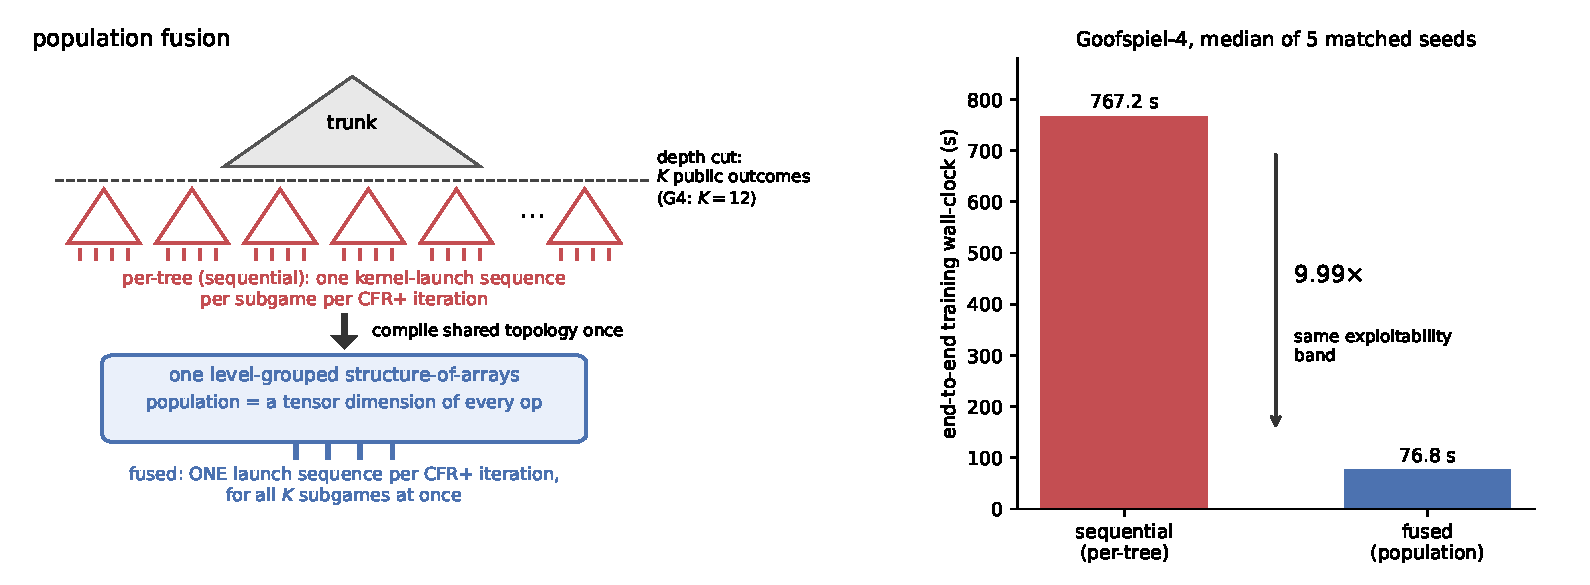
\includegraphics[width=\linewidth]{figs/fig_hero.pdf}
\caption{\textbf{Population fusion, and what it buys end to end.} \emph{Left:} at the
depth cut, the \emph{trunk} --- the above-cut portion of the game, which the agent
solves directly and whose leaf values the subgame population provides --- has $K$ public
outcomes, each rooting a same-topology subgame (G4:
$K = 12$); solved per-tree, each subgame costs its own kernel-launch sequence per CFR+
iteration. Population fusion compiles the shared topology once into a level-grouped
structure-of-arrays and folds the population into a tensor dimension of every op, so one
launch sequence per CFR+ iteration solves all $K$ subgames. \emph{Right:} end-to-end
Goofspiel-4 training wall-clock, median of 5 matched seeds: sequential 767.2 s vs fused
76.8 s --- 9.99$\times$, with no gross divergence under the descriptive band check
(\S6.2). The tool-symmetric compile-vs-compile check gives 7.38$\times$ total-wall
speedup (\S6.5).}
\label{fig:hero}
\end{figure}

\subsection*{Contributions}

\begin{itemize}
\item \textbf{Identification of the population structure as a cost-per-solve lever.}
Train-time iterated resolving structurally generates, at every iteration, a population
of $K$ same-topology depth-limited PBS subgames differing only in entry beliefs, and
amortizing cost-per-solve across that population is, to our knowledge, not isolated and
validated end to end in published work (\S3, \S7). The lever is orthogonal in form to
the four claimed levers of Eq.~(\ref{eq:cost}); composition with them is untested
(\S8).
\item \textbf{A parity-verified fused solver.} Population fusion compiles the shared
topology once into a level-grouped, flat structure-of-arrays CFR+ and runs each
iteration of \emph{all} subgames as one fixed sequence of batched tensor ops, recovering
classical range-vector semantics across heterogeneous decision/chance/variable-action
structure and across public keys. It matches the per-tree finite-iteration CFR+ average
strategies and leaf values, in the verified sense defined by the gates of \S5
(Proposition~1, \S4.5).
\item \textbf{A predictive floor/slope cost model with a two-point regime probe.}
The model is
$C_{\rm seq}(N)=a_s+b_s(N-1)$ and
$C_{\rm fus}(N)=a_f+b_f(N-1)$: near-linear while the fused marginal slope is near zero,
and slope-ratio-limited once one subgame fills the device. The
$\min(N,1/\varphi)$ form remains the launch-bound envelope and regime intuition
(\S6.1). The microbenchmark prediction transfers to the live training loop at both ends
(\S6.2, \S6.4).
\item \textbf{An Amdahl-surviving end-to-end training win.} In a tabula-rasa self-play
resolving loop on Goofspiel-4 (5 matched seeds, one configuration fixed in advance),
tool-symmetric compile-vs-compile fusion gives 11.36$\times$ inner and 7.38$\times$
total-wall speedup against a 7.39$\times$ Amdahl ceiling. The eager-dispatch isolate
gives 11.79$\times$ inner and 9.99$\times$ total wall-clock speedup (fused median 76.8 s
vs sequential 767.2 s) against a 10.09$\times$ Amdahl ceiling. The sequential arm is a
same-kernel per-tree GPU baseline analogous to within-tree GPU-CFR~\citep{Kim2024}; it
is not Kim's implementation or NoRegret. Both comparisons make no lower-exploitability
claim and are gated by the broad descriptive band check (\S6.2, \S6.5).
\item \textbf{A finding about evaluating batched GPU game solvers.} CUDA atomics
compound through CFR training into per-seed final-exploitability divergences far larger
than any reasonable per-seed tolerance, so naive per-seed equivalence checks of batched
GPU CFR through a training loop will spuriously fail. The remedy is part of the method:
gate algorithmic equivalence on CPU, where the two arms are exactly the same algorithm,
and use GPU runs for timing and band-level comparison only (\S5, \S6.2).
\end{itemize}

\begin{table}[t]
\centering
\small
\caption{\textbf{Novelty boundary.} The contribution is the validated conjunction in
the last row, not batching or GPU-CFR in isolation.}
\label{tab:novelty}
\begin{tabular}{>{\raggedright\arraybackslash}p{0.27\linewidth}
                >{\raggedright\arraybackslash}p{0.29\linewidth}
                >{\raggedright\arraybackslash}p{0.34\linewidth}}
\toprule
Line of work & What it parallelizes or amortizes & Boundary relative to this paper \\
\midrule
GPU-CFR / NoRegret~\citep{Kim2024,KimSandholm2026} & One extensive-form tree's CFR
iteration, reframed as linear algebra & Our sequential arm is the same-kernel per-tree
analogue; the new axis is a population of same-topology subgames from one resolving
sweep. \\
Real-Time Parallel CFR~\citep{RealTimeParallelCFR} & One large HUNL depth-limited solve
through CPU/GPU pipeline stages, pruning, abstraction, and GPU leaf evaluation & A
single-solve real-time pipeline; orthogonal to same-topology population fusion. \\
DeepStack/ReBeL-style resolving~\citep{Moravcik2017,Brown2020} & Learned value leaves
and public-belief search/resolving & Supplies the workload family; solve-kernel
population fusion is not isolated there. \\
Distributed subgame solving~\citep{Bowling2015,Tammelin2015} & Independent subgames
over distributed workers & Task parallelism across workers, not one fused
single-device kernel-launch sequence. \\
This work & All same-topology cut subgames in one resolving sweep & Parity-gated fused
CFR+ iteration, predictive regime model, and end-to-end timing validation. \\
\bottomrule
\end{tabular}
\end{table}

\section{Background}

This section teaches the three prerequisites the rest of the paper assumes: how CFR+
solves an imperfect-information game (\S2.1), what depth-limited resolving and public
belief states are and where the population of subgames arises (\S2.2), and why many
small GPU workloads are slow (\S2.3). It closes with the paper's notation and project
vocabulary. Readers fluent in CFR and GPU performance can skim directly to
Table~\ref{tab:notation}.

\subsection{Extensive-form games, regret, and CFR+}

A two-player zero-sum \emph{extensive-form game} is a game tree with three kinds of
nodes: decision nodes, where one player acts; chance nodes, where nature acts with known
probabilities (a card is dealt, a prize is revealed); and terminals, which pay out.
Hidden information is modeled by \emph{information sets} (infosets): an infoset collects
all the tree states a player cannot distinguish given what they have observed, and the
player must act identically across them. A \emph{strategy} $\sigma$ assigns each infoset
a probability distribution over its actions. A \emph{Nash equilibrium} is a strategy
profile in which neither player can gain by deviating; \emph{exploitability} measures
distance from it in plain terms --- how much an optimal opponent could gain against the
strategy. Zero means exact Nash; on Goofspiel-4, the running example introduced below,
uniform random play scores $\approx$1.42. (The formal metric, NashConv, is defined in
\S5.)

Counterfactual Regret Minimization (CFR)~\citep{Zinkevich2007} solves such games by
iterated self-play over the regrets of actions. The \emph{regret} of an action at an
infoset is how much better that action would have done than the current strategy, in
hindsight, weighted by the \emph{counterfactual reach} --- the probability that the
opponent and chance alone would bring play to this infoset. (The player's own
contribution to reaching the infoset is divided out; that is what ``counterfactual''
means.) \emph{Regret matching}~\citep{HartMasColell2000} turns accumulated regrets into
the next strategy: play each action with probability proportional to its positive
cumulative regret --- a clamped normalization. Every CFR variant shares one iteration
structure: \textbf{(1)} regret-match the current strategy from the regret table;
\textbf{(2)} a \emph{forward pass} propagates reach probabilities from the root to the
leaves; \textbf{(3)} a \emph{backward pass} propagates expected values from the leaves
to the root, depositing per-action regret contributions at each infoset; \textbf{(4)}
update the cumulative-regret table and an average-strategy table. The convergence fact
that drives everything: it is the \emph{time-averaged} strategy --- not the last iterate
--- that converges to a Nash equilibrium, at rate $O(1/\sqrt{T})$ in the iteration count
$T$, which is why an average-strategy table $S$ is carried alongside the regret table
$R$. CFR+~\citep{Tammelin2014} is the practical workhorse variant: it clamps cumulative
regrets at zero (so an action that has done badly can re-enter quickly), alternates
which player updates each iteration, and weights the average linearly toward later
iterates~\citep{Tammelin2015,BurchMoravcikSchmid2019}.

\textbf{A worked mini-example.} Table~\ref{tab:toy} runs three CFR+ iterations at a
single infoset with two actions $\{a, b\}$, holding the counterfactual reach at $0.5$.
\emph{All numbers in Table~\ref{tab:toy} are pedagogical toys, not measurements};
strategy entries are rounded to two decimals, and the rounded values are used in the
next row's arithmetic so the table is self-contained (the average-strategy accumulation
is omitted for compactness).

\begin{table}[t]
\centering
\caption{Three toy CFR+ iterations at one infoset (\textbf{illustrative numbers only}).}
\label{tab:toy}
\small
\begin{tabular}{cllclcl}
\toprule
iter & $R = (R_a, R_b)$ & $\sigma \propto [R]_+$ & $v(a), v(b)$ & $v(\sigma)$ & deltas $\times\,0.5$ & new $R$ \\
\midrule
1 & (6.00, 2.00) & (0.75, 0.25) & $1,\ 3$ & 1.50 & $(-0.25, +0.75)$ & (5.75, 2.75) \\
2 & (5.75, 2.75) & (0.68, 0.32) & $2,\ -3$ & 0.40 & $(+0.80, -1.70)$ & (6.55, 1.05) \\
3 & (6.55, 1.05) & (0.86, 0.14) & $1,\ -4$ & 0.30 & $(+0.35, -2.15)$ & (6.90, \textbf{0.00}) \\
\bottomrule
\end{tabular}
\end{table}

Read row 1: cumulative regrets $(6, 2)$ regret-match to $\sigma = (0.75, 0.25)$; this
iteration's counterfactual action values are $v(a) = 1$ and $v(b) = 3$, so the infoset
is worth $0.75 \cdot 1 + 0.25 \cdot 3 = 1.5$ under $\sigma$; each action's regret delta
is its value minus the infoset value, scaled by the counterfactual reach $0.5$, giving
new cumulative regrets $(5.75, 2.75)$ and hence next strategy $(0.68, 0.32)$. In row 3,
action $b$'s running total goes negative ($1.05 - 2.15 = -1.10$) and CFR+ floors it at
zero --- the clamp --- after which $b$ is played with probability 0 but can re-enter as
soon as it accumulates positive regret again. The four-step skeleton --- (1)
regret-match, (2) forward reach, (3) backward counterfactual values, (4) regret/average
update --- is exactly what \S4.3 turns into four batched tensor operations.

\subsection{Depth-limited resolving, public belief states, and where the population arises}

Vocabulary first. \emph{Public} information is observed by both players: revealed cards,
bids, the board, the betting so far. \emph{Private} information is a player's hidden
holding. The \emph{reach probability} of a state under a strategy profile is the product
of the action probabilities along the path to it. A player's \emph{range} at a public
state is a probability vector over that player's possible private states --- what an
observer who saw only the public actions should believe the player holds. A \emph{public
belief state} (PBS) packages exactly this:
\[ \beta = \big(s_{\text{pub}},\, (r_1, r_2)\big), \]
a public state $s_{\text{pub}}$ together with each player $i$'s range $r_i$ over their
private states consistent with $s_{\text{pub}}$~\citep{Brown2020}. In poker, $\beta$ is
the community cards and betting history plus each player's distribution over hole cards.
In our running example it is the following.

\textbf{Running example: Goofspiel.} In Goofspiel-$k$~\citep{Ross1971} each player holds
a hand of $k$ cards, valued $1$ to $k$, used as sealed bids (Goofspiel-4, ``G4'': $k =
4$). Each round a prize card is revealed, in an order chosen at random; both players
simultaneously bid one card from their hand; the higher bid takes the prize. Players
observe who won the round but not the opponent's bid card, so the opponent's spent ---
hence remaining --- cards are hidden: the hidden hand is the private state, and the
prize sequence plus the per-round win/loss/tie outcomes are the public state. We place
the depth-limit cut at the chance boundary where the second prize is about to be
revealed --- i.e., after the first resolved round. The public information there is which
prize was contested and how the bid comparison went, taking $K = 4 \times 3 = 12$
distinct values at G4 (9 at G3, 15 at G5). Each of these $K$ \emph{public keys} roots an
identically shaped continuation subgame, because the remaining structure of the game
depends only on how many cards remain, not which. Each key's subgame carries the hidden
bid pairs consistent with its outcome as private-deal instances; summed over keys these
give $B = 64$ \emph{cut instances} at G4 (27 at G3, 125 at G5).

\textbf{Why naive depth limits are unsound.} Truncating the lookahead and valuing cut
nodes with belief-blind numbers fails in imperfect-information games: the value of a cut
node depends on what both players believe about the hidden information --- a poker leaf
is worth more when your range is credibly strong --- so a leaf must be valued
conditional on the belief pair. Value the cut with belief-blind numbers and the solver
above the cut learns strategies a real opponent exploits~\citep{BrownSandholm2018}. The
sound instantiations --- DeepStack's continual re-solving~\citep{Moravcik2017},
ReBeL~\citep{Brown2020}, Student of Games~\citep{Schmid2023} --- train a value network
$\hat V(\beta)$ over PBSs and re-solve subgames at play time and, critically for this
paper, at \emph{train} time; value-function error propagates to exploitability with
known bounds~\citep{KovarikLisy2019}.

\textbf{The training loop.} The tabula-rasa loop we accelerate is iterated continual
resolving with \emph{per-belief finite-budget CFR+ targets}: in each round, (i) sample a
belief $\beta$ at every cut public state; (ii) \textbf{run the fixed CFR+ budget on
every below-cut subgame at the sampled belief} and read off the normalized continuation
values $V_T(\beta)$; (iii) regress the PBS value net on $(\beta, V_T(\beta))$ rows; (iv)
periodically re-solve the trunk (the above-cut portion of the game, which the agent
solves directly; Figure~\ref{fig:hero}) against the current net leaf and measure
exploitability of the assembled policy. Step (ii) is the \emph{inner re-solve} and is where the cost
lives. Leaf values use a fixed \emph{normalized} PBS convention,
\[ v_i(h_i \mid \beta) \;=\; \frac{\sum_{h_{-i}} r_{-i}(h_{-i})\, \mathrm{EV}_i(h_i,
h_{-i})}{\sum_{h_{-i}} r_{-i}(h_{-i})}, \]
where $h_i$ ranges over player $i$'s private states consistent with $s_{\text{pub}}$,
$r_{-i}$ is the opponent's entry reach vector of $\beta$, and $\mathrm{EV}_i(h_i,
h_{-i})$ is player $i$'s expected continuation payoff at the cut instance identified by
the private pair $(h_i, h_{-i})$ --- under the re-solved subgame's average strategy when
generating targets, and under the exact full-game continuation in the round-trip
validation. The convention is validated by a round-trip gate: valuing the trunk through
this leaf interface reproduces exact full-game above-cut values to $\sim 10^{-15}$ (the
gate mechanics and the zero-reach edge case are in Appendix~A).

\begin{algorithm}[t]
\caption{Iterated resolving with population-fused target generation}
\label{alg:trainingloop}
\begin{algorithmic}[1]
\For{training round $r=1,\dots,R$}
  \State sample PBS beliefs $\beta_{j,k}$ for each training belief $j$ and cut public
         key $k$
  \For{belief sample $j$}
    \State solve all $K$ below-cut subgames at $\{\beta_{j,k}\}_{k=1}^K$ for fixed CFR+
           budget $T$
           \Comment{sequential: host loop over $k$; fused: one population solve}
    \State extract normalized finite-budget targets $V_T(\beta_{j,k})$
  \EndFor
  \State update value net on the collected $(\beta,V_T(\beta))$ rows
  \State periodically solve the trunk against the current value net and score exact
         NashConv
\EndFor
\end{algorithmic}
\end{algorithm}

\textbf{Where the population arises.} The inner re-solve is never one subgame: a single
belief sample requires solving \emph{all} $K$ keys' subgames at once, and target
generation repeats that $K$-population solve for every sampled belief in every round.
This is a representative workload of the method family --- DeepStack's value networks were
trained on the order of $10^7$ independently re-solved subgames~\citep{Moravcik2017}.
Kim \& Sandholm make the mirror observation from the within-tree side: their GPU-CFR
framework is particularly useful for ``games that are played in a repeated setting,
whose individual game trees usually differ by little to none across
repetitions''~\citep{KimSandholm2026} --- the population of same-topology subgames is
the train-time analogue of that observation, taken across the subgames of one resolving
sweep rather than across episodes.
One central delimitation for the novelty claim: \emph{within} a key, solving for
all private-deal instances simultaneously is the classical range-vector decomposition of
CFR~\citep{Johanson2011,Johanson2012}, used in DeepStack's own resolver and carried
identically by \emph{both} of our timing arms; the \emph{across-key} axis $K$ is what
this paper adds (full delimitation in \S4.5 and \S7).

\subsection{GPU execution economics}

The last prerequisite is the cost structure of GPU execution, for the reader who knows
ML but not GPU performance. Every kernel launch costs a fixed amount of host-side
overhead --- on the order of microseconds --- regardless of how much work the kernel
does. A workload made of many small kernels is therefore \emph{launch-bound}: the device
idles between launches, and throughput is set by the host's ability to feed it, not by
arithmetic. This launch-bound regime is, we believe, the same phenomenon Kim \&
Sandholm~\citep{KimSandholm2026} report from the other side: their GPU
implementation is slower than OpenSpiel's C++ on small games (Kuhn and Leduc poker),
where kernel-launch overhead dominates useful work. Throughout, \emph{eager dispatch}
means each tensor operation is issued to the GPU as its own kernel launch the moment the
Python interpreter reaches it, in contrast to captured or compiled execution, which
records a kernel sequence once and replays it. A workload whose individual kernels fill
the device is \emph{saturated}
(compute-bound) and gains nothing from more concurrency. Batching many same-shaped small
problems into one kernel --- so the device does the same arithmetic under $O(1)$
launches --- is the founding insight of batched
BLAS~\citep{Abdelfattah2016,Abdelfattah2021}, and roofline-style throughput
arithmetic~\citep{Williams2009} frames the cost model we build in \S6.1. CUDA
Graphs~\citep{CUDAGraphs} are the rival lever: record a fixed kernel sequence once, then
replay it with a single launch --- amortizing launch cost without fusing any work (we
analyze this alternative for our kernel in \S4.6). Finally, define the \emph{fill
fraction} $\varphi \in (0, 1]$ informally as the fraction of the device one subgame's
kernels occupy: roughly $1/\varphi$ such subgames fit before the device saturates. This
is all a reader needs to predict the two-regime model of \S6.1: co-solving $N$ subgames
should pay about $N\times$ while $N \lesssim 1/\varphi$, and plateau beyond.

\textbf{Notation and project vocabulary.}

\begin{table}[t]
\centering
\caption{Notation.}
\label{tab:notation}
\small
\begin{tabular}{ll}
\toprule
symbol & meaning \\
\midrule
$K$ & public keys at the cut --- the across-solve fusion axis \\
$B$ & cut instances: private-deal combinations, summed over keys \\
$N$ & number of co-solved subgames in controlled sweeps \\
$\varphi$ & fill fraction: fraction of the device one subgame's kernels occupy \\
$m$ & fused marginal-cost probe value (\S6.1) \\
$N^* \approx 1/m$ & regime boundary estimated by the probe \\
$f$ & inner-resolve fraction of the baseline loop's wall-clock \\
$S_{\text{inner}}$ & fused-vs-sequential inner-resolve speedup \\
$T$ & CFR+ iterations per solve \\
$c_{\text{solve}}$ & wall-clock per solve-iteration \\
$n_I$ & below-cut infosets (rows of the regret table) \\
$A_{\max}$ & maximum actions per infoset (padded) \\
$R,\ S,\ \sigma$ & cumulative-regret table, strategy-sum table, current strategy \\
\bottomrule
\end{tabular}
\end{table}

Three project terms used from the abstract on: a \textbf{gate} is a hard pass/fail check
run as part of the experiment pipeline (``verified/gated at $x$'' = certified to $x$ by
such a check); the two \textbf{arms} of an experiment are the two runs sharing one seed
--- fused and sequential --- in the clinical-trial sense; \textbf{equal-band-faster} is
this paper's claim form --- the same final exploitability band, in less wall-clock.

There are two population dimensions in the implementation. $K$ is the conceptual
across-solve axis: the number of public-key subgames one resolving sweep must solve.
$B$ is the flattened cut-instance dimension after each key's compatible private-deal
rows are expanded. The implementation carries $B$ in tensor axes, while the cost model
varies the number of co-solved public-key subgames as $N$.

\section{The Cost of Iterated Resolving}

Before describing the mechanism, we quantify the problem it solves. The three facts
below are measured in the experiments of \S6 (artifacts in \S10); this section states
each once, in its motivating role.

\textbf{Fact 1 --- the loop \emph{is} the inner solve.} In our instrumented training
runs, the inner re-solve (step (ii) of the \S2.2 loop) accounts for \textbf{98.4\%} of
baseline loop wall-clock at the Goofspiel-4 operating point, and \textbf{86.1\%} at
Goofspiel-5 (median of 3 quiet-host seeds; \S6.2, \S6.4). By Amdahl's
law~\citep{Amdahl1967}, accelerating the inner re-solve is, to first order, accelerating
training itself.

\textbf{Fact 2 --- the GPU is starving, not slow.} At Goofspiel-4 scale, eager per-tree
GPU dispatch is $\sim$\textbf{4.3$\times$ slower} per belief than the same kernel run on
the host CPU (GPU-sequential 2.353 s vs CPU-sequential 0.547 s per
belief).\footnote{The CPU cells are single determinism-gate runs without warmup/repeat
discipline, so the cross-substrate readings are provisional on matched
full-configuration CPU timings; the full 2$\times$2, its provenance, and its caveats are
in \S4.6 and Appendix~C.} Small float64 subgames pay for kernel launches, not arithmetic
--- solved one tree at a time, the GPU loses to its own host. The same artifacts set the
paper's cross-substrate floor: against the strongest non-fused arm we measured (the same
kernel, sequential, on the host CPU), the best-vs-best Goofspiel-4 win for the fused GPU
solver is $\sim$\textbf{2.7$\times$} (\S4.6).

\textbf{Fact 3 --- fusion removes the per-subgame launch cost.} Fused solve time is
essentially \textbf{flat in the number of co-solved public-key subgames} --- 197.6
$\to$ 202.4 ms as the Goofspiel-4 sweep size goes $1 \to 12$ --- while sequential per-tree time
grows linearly (\S6.1). Added subgames ride along nearly free until the device fills.

\textbf{The lever taxonomy, compressed.} Prior work claims every factor of
Eq.~(\ref{eq:cost}) except the one Facts 2 and 3 point at. $N_{\text{solves}}$ is
reduced by TurboReBeL's single-sample multi-iteration data
generation~\citep{TurboReBeL}; $T$ by regret-minimizer design --- DCFR/PCFR+ and the
meta-learned predictive minimizers, deployed on each subgame
sequentially~\citep{BrownSandholm2019,Farina2021,Sychrovsky2024,NPCFR}; sampling
variance by the MCCFR
family~\citep{Lanctot2009,Schmid2019,McAleer2023,Steinberger2020}; subgame size by
learned abstractions~\citep{LAMIR}. The remaining factor, $c_{\text{solve}}$, has been
attacked only \emph{within} a single tree, by the GPU-CFR
line~\citep{Kim2024,KimSandholm2026}. The cost-per-solve-across-the-population axis ---
making each CFR+ iteration cheaper by amortizing it over many subgames at once, exactly
--- is not isolated in prior published work as an end-to-end population-level lever;
\S7 gives the lever-by-lever discussion and the
related-work delimitation.

\section{Method: Population Fusion}

\subsection{Mechanism overview}

The whole mechanism is three sentences. (1) All $K$ cut subgames share one topology,
differing only in data --- entry reaches, payoffs, infoset identities (\S2.2). (2) We
compile that topology \emph{once} into a flat structure-of-arrays layout whose nodes are
grouped by level and shape (\S4.2). (3) Each CFR+ iteration of \emph{all} subgames then
executes as one fixed sequence of batched tensor ops (\S4.3): the population axis moves
from a host-side loop --- one kernel-launch sequence per subgame --- into the innermost
tensor dimension of every op, so the per-iteration launch count is
$O(\#\text{level-shape groups})$, independent of the co-solved public-key count.
Figure~\ref{fig:walkthrough} walks the mechanism through a tiny two-subgame example, and
Algorithms~\ref{alg:seq} and~\ref{alg:fused} state the two timing arms side by side:
identical four steps, identical kernels, differing in exactly one line. (Shape
annotations in Algorithm~\ref{alg:fused}: $G$ is the node count of the level-shape group
an op ranges over, $A$ the group's per-infoset action count, and $B$ the flattened
cut-instance dimension of \S2.2; full notation in \S4.3.)

\begin{figure}[t]
\centering
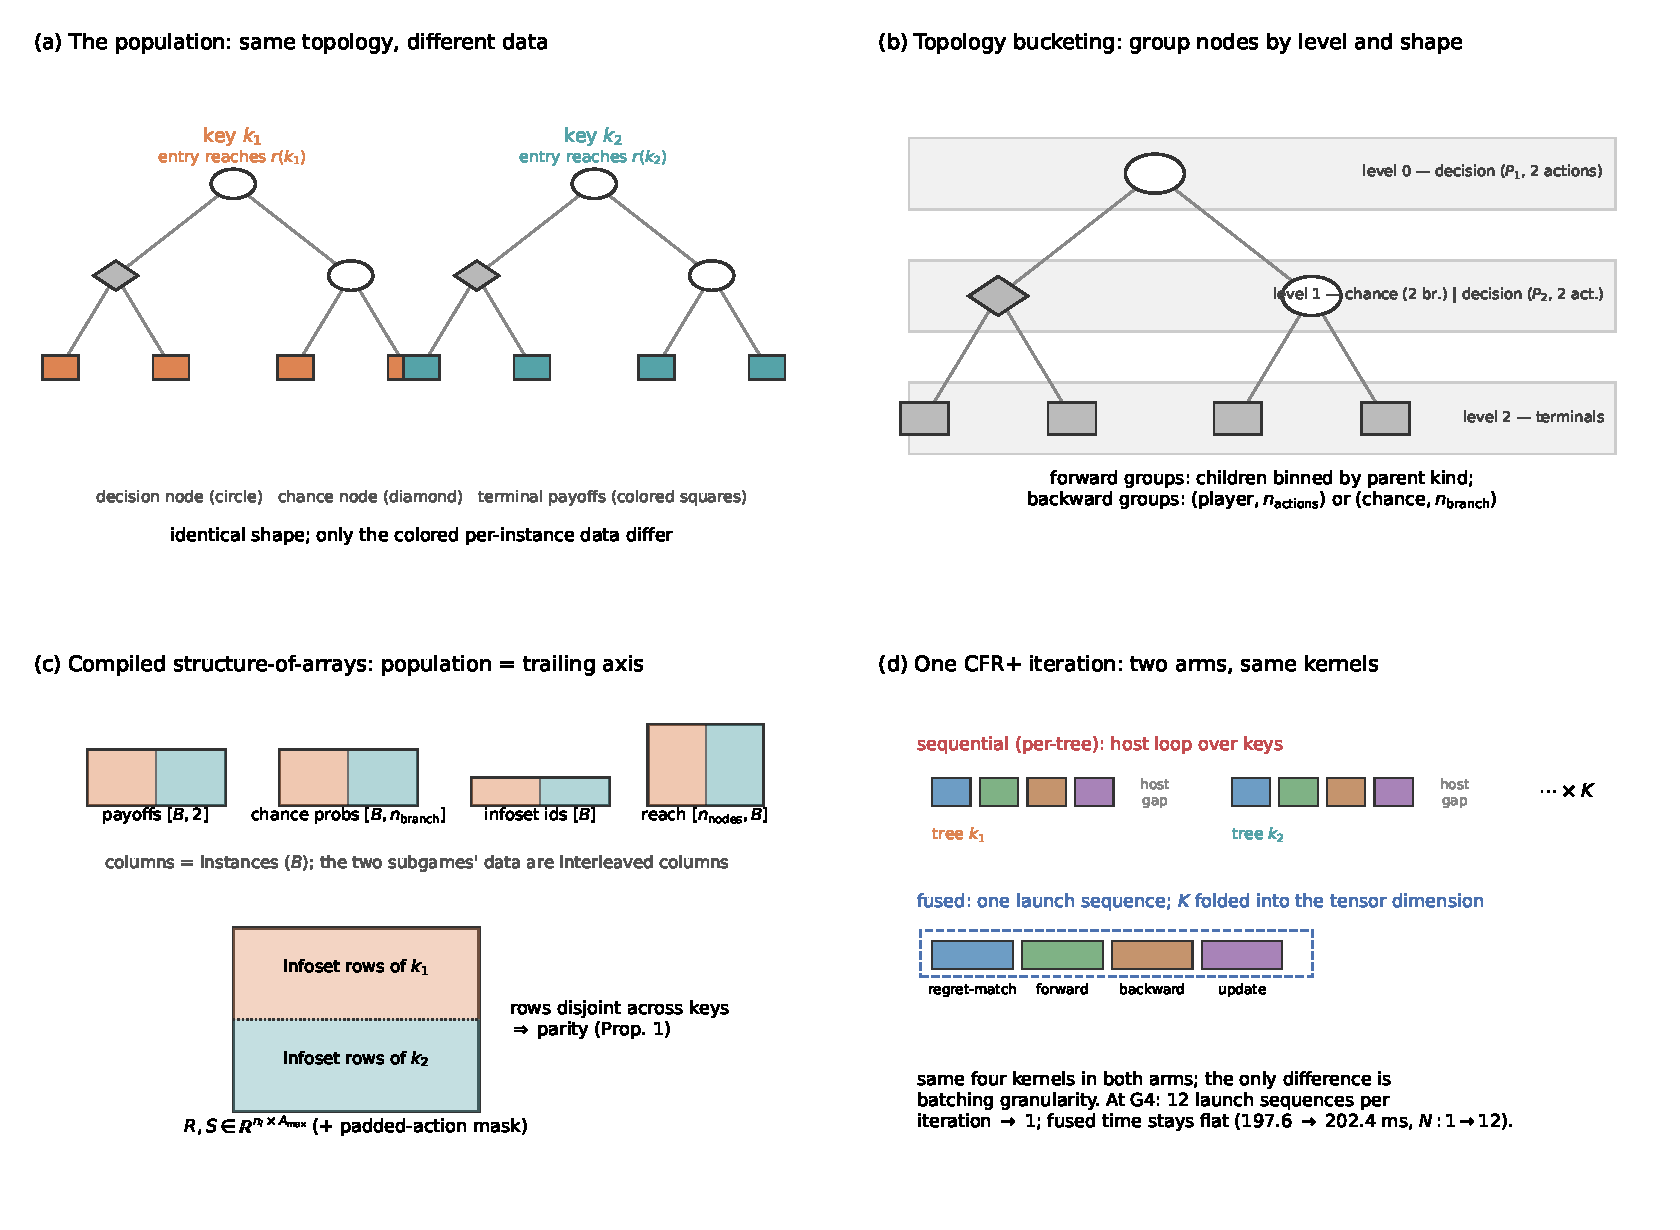
\includegraphics[width=\linewidth]{figs/fig_walkthrough.pdf}
\caption{\textbf{Population fusion on a tiny two-subgame example.} \emph{(a)} Two
same-topology depth-limited subgames rooted at public keys $k_1, k_2$ on the trunk's cut
frontier; per-instance data (entry reaches, terminal payoffs) shown in color --- same
shape, different data. \emph{(b)} The same topology drawn once, with nodes binned into
level-shape groups: forward groups keyed by parent kind, backward groups keyed by
(player, $n_{\text{actions}}$) or (chance, $n_{\text{branch}}$). \emph{(c)} The compiled
structure-of-arrays: per-node data become length-$B$ arrays with the population as the
trailing axis, and the global regret/strategy-sum tables $R, S \in \mathbb{R}^{n_I
\times A_{\max}}$ hold the two keys' infoset rows as disjoint blocks --- visually
pre-stating the parity argument of \S4.5. \emph{(d)} One CFR+ iteration as kernel
timelines: the sequential arm issues one launch sequence per tree with host gaps between
them; the fused arm issues one launch sequence total, with $K$ folded into the tensor
dimension. At G4 this is 12 launch sequences per iteration $\to$ 1, and fused time stays
flat as the population grows (197.6 $\to$ 202.4 ms for $N{:}\,1{\to}12$; \S6.1).}
\label{fig:walkthrough}
\end{figure}

\begin{algorithm}[t]
\caption{Per-tree CFR+ (the sequential arm)}
\label{alg:seq}
\begin{algorithmic}[1]
\State compile each key $k$'s topology once (shared shape, per-key data)
\For{$t = 1, \dots, T$} \Comment{one CFR+ iteration}
  \For{$k = 1, \dots, K$} \Comment{\textbf{host loop: one launch sequence per tree}}
    \State \textbf{regret-match:} $\sigma_k \gets \text{clamp-normalize}(R_k)$
    \State \textbf{forward pass:} reaches root $\to$ leaves on tree $k$
    \State \textbf{backward pass:} counterfactual values leaves $\to$ root; deposit
           regret contributions into $R_k$
    \State \textbf{CFR+ update:} clamp $R_k$ at $0$; alternate player; update $S_k$
  \EndFor
\EndFor
\end{algorithmic}
\end{algorithm}

\begin{algorithm}[t]
\caption{Fused population CFR+ (this work)}
\label{alg:fused}
\begin{algorithmic}[1]
\State compile the shared topology once (population data: length-$B$ arrays)
\For{$t = 1, \dots, T$} \Comment{one CFR+ iteration: \textbf{one launch sequence;
      the population is a tensor dimension}}
  \State \textbf{regret-match:} $\sigma \gets \text{clamp-normalize}(R)$
         \Comment{all legal rows at once; pad slots masked}
  \State \textbf{forward pass:} batched gather $\times$ multiply over level groups
         \Comment{$[G, B]$ blocks}
  \State \textbf{backward pass:} batched contractions + scatter-add
         \Comment{$[G, A, B, 2]$ by per-instance infoset id}
  \State \textbf{CFR+ update:} clamp at $0$; alternate player; update $S$
         \Comment{masked average-strategy normalization}
\EndFor
\end{algorithmic}
\end{algorithm}

The two algorithms run the same kernels on the same data; they differ in exactly one
visible line --- the host loop over keys versus the population tensor dimension. This is
also the baseline-fairness claim of \S4.6 in pictorial form: the sequential arm is not a
weak baseline but the identical kernel at a different batching granularity.

\subsection{Topology compilation}

Our subgame-construction layer (\texttt{DepthLimitedGame}) enumerates an OpenSpiel
game~\citep{Lanctot2019} once into a tagged tree of terminal, chance, decision, and
\textbf{cut} nodes; the cut predicate is the one game-specific hook, and each cut node
records its public key $k$, each player's private index $(i_0, i_1)$ at that key, and
the continuation subtree. Compilation then proceeds in four steps. \textbf{(1)} Tag the
shared below-cut topology from the cut nodes (the cut sits at a public chance boundary,
so instances differ only in private deals --- hence in entry reaches, payoffs, and
infoset identities, not in shape). \textbf{(2)} One recursive descent over the
\emph{lockstep population} --- all $B$ instances advanced through the shared topology
together --- emits one record per topology node whose per-instance data are length-$B$
arrays: terminal payoffs $[B, 2]$, chance branch probabilities $[B,
n_{\text{branch}}]$, and per-instance global infoset ids $[B]$ at decision nodes.
\textbf{(3)} Group the records \textbf{by level and shape}: forward groups collect all
level-$L$ children by parent kind (decider 0, decider 1, chance); backward groups
collect all level-$L$ non-terminals by $(\text{player}, n_{\text{actions}})$ or
$(\text{chance}, n_{\text{branch}})$. \textbf{(4)} Absorb variable depth, heterogeneous
branching factors, and interleaved chance nodes into these groups plus padded
legal-action masks over the union of below-cut infosets. A reimplementer must get three
things right: the global infoset-id space spans the whole population (it indexes the
rows of $R$); the ids are \emph{per-instance}, so the same topology node maps to
different rows in different instances; and pad slots must be masked out of every
subsequent update.

\subsection{The fused CFR+ iteration}

What one CFR+ iteration computes, in the vocabulary of \S2.1: step 1 turns accumulated
regrets into the \emph{current} strategy --- the clamped normalization of regret
matching. Step 2 pushes \emph{reach probabilities} from the entry reaches down to every
node --- ``how likely is play to get here, and who contributed''. Step 3 pulls
\emph{expected values} from the terminals back up, forming counterfactual action values
weighted by opponent-and-chance reach, and deposits each infoset's regret contributions.
Step 4 is the CFR+ update: clamp cumulative regrets at zero, alternate the updating
player, and accumulate the own-reach-weighted average strategy --- the quantity whose
time average converges to equilibrium. Fused, each step becomes one batched operation
per level-shape group.

\emph{Notation:} $B$ cut instances and $K$ public keys as in \S2.2; $n_I$ below-cut
infosets in the population union with at most $A_{\max}$ actions each; $R, S \in
\mathbb{R}^{n_I \times A_{\max}}$ the global regret and strategy-sum tables; $\sigma$
the current strategy from regret matching; $r^{\text{own}}, r_{-i}, r^c$ own, opponent,
and chance reaches; $G$ as defined in the Algorithm~\ref{alg:fused} gloss (\S4.1).
Each CFR+ iteration is a fixed sequence of batched tensor ops with \emph{no
per-iteration Python tree recursion}:

\begin{enumerate}
\item \emph{Regret matching}~\citep{HartMasColell2000}\emph{:} one clamped-normalize
over the global regret table $R$ (float64), $\sigma(I,a) = [R(I,a)]_+ / \sum_{a'}
[R(I,a')]_+$ over legal actions, uniform over legal actions where the denominator
vanishes (illegal slots are mask-padded out of every update).
\item \emph{Forward reach pass:} for each forward group, child reaches are one gather +
elementwise multiply --- $r^{\text{own}}_{\text{child}} = r^{\text{own}}_{\text{parent}}
\odot \sigma[\text{id}, \text{slot}]$ for decision parents, where $\sigma[\text{id},
\text{slot}]$ is the parent infoset's current-strategy entry for the action leading to
the child, and $r^c_{\text{child}} = r^c_{\text{parent}} \odot p$ for chance parents,
where $p$ is the branch probability --- over $[G, B]$ blocks.
\item \emph{Backward value pass:} for each backward group, child EVs are gathered as
$[G, A, B, 2]$ tensors, where $A$ is the group's per-infoset action (or chance-branch)
count, and contracted against $\sigma$ (or chance probabilities); counterfactual action
values $r_{-i}\, r^c\, \mathrm{EV}$ (opponent reach times chance reach --- the
counterfactual reach) are scattered into the global accumulator with
\texttt{index\_add\_} over the per-instance infoset ids.
\item \emph{CFR+ update:} alternating-player regret update with clamp at zero,
own-reach-weighted strategy sums, linear averaging (on the interaction of alternating
updates with averaging in CFR+, see~\citep{BurchMoravcikSchmid2019}).
\end{enumerate}

Per-iteration kernel-launch and op count is $O(\#\text{level-shape groups})$ --- fixed
by the topology and \emph{independent of the co-solved public-key count}, which appears only as a
tensor dimension (the arithmetic work per op scales with it, which is precisely what
fills the device). In the work--depth vocabulary of~\citep{KimSandholm2026}, the
population enters the \emph{work}, not the \emph{depth}: per-iteration work scales
linearly with the cut-instance tensor dimension, while the launch/op count --- the host-side serial
term --- stays $O(\#\text{level-shape groups})$, independent of it. (We use
``GEMM-shaped'' --- GEMM: general matrix--matrix multiplication --- loosely, here and in
the title: the per-iteration ops are gathers, scatters, and elementwise products plus
small dense contractions, executed as batched tensor kernels.) Running example, one G4 resolve
sweep: $K = 12$ keys, $B = 64$ instances, 300 CFR+ iterations --- the sequential arm
issues 12 launch sequences per iteration $\times$ 300 iterations; the fused arm issues
one per iteration.

\begin{table}[t]
\centering
\caption{\textbf{Per-CFR-iteration operation structure.} $L$ is the number of
level-shape groups, $K$ the public-key population size, and $B$ the flattened
cut-instance tensor dimension. Arithmetic work scales with the population in both views;
fusion removes the host-side serial launch sequence over keys.}
\label{tab:opcount}
\begin{tabular}{p{0.24\linewidth}p{0.31\linewidth}p{0.34\linewidth}}
\toprule
Quantity & per-tree sequential arm & fused population arm \\
\midrule
Host launch sequences per CFR+ iteration & $K L$ & $L$ \\
Tensor arithmetic work & $\Theta(B \cdot \text{group work})$ across $K$ calls &
$\Theta(B \cdot \text{group work})$ in one batched call \\
Regret / strategy rows & disjoint per key & union table $R,S\in\mathbb{R}^{n_I\times A_{\max}}$ \\
Serial host loop over public keys & yes & no \\
Correctness condition & per-key CFR+ & same update plus disjoint below-cut rows \\
\bottomrule
\end{tabular}
\end{table}

\subsection{Reuse across resolves, and the value pass}

Between solves only the entry reaches change: the two $[B]$ entry-reach vectors are
rewritten and the compiled topology is reused for the whole training run. Compilation is
one-time infrastructure and is excluded from all solve timings symmetrically in both
arms --- conservatively for the fused claim, since the sequential arm requires $K$
per-key compiles plus the shared one (the corresponding setup costs are: topology
compile 0.09--9.4 s per game,
\texttt{torch.compile} $\le$9.3 s, CUDA-Graph capture $\le$0.15 s --- all excluded
symmetrically). After the final iteration, a
value-only backward pass under the average strategy returns the per-instance
continuation EV $\text{cont} \in \mathbb{R}^{B \times 2}$, from which normalized
per-private leaf values (\S2.2) are reconstructed in $O(B)$ --- so target generation and
trunk leaf queries also avoid any Python subtree walk.

\subsection{Parity: the fused solve matches finite-iteration CFR+ outputs}

We require the fused solve to return the same finite-iteration CFR+ average strategies
and leaf values as the per-tree solve --- exact in the verified sense defined by the
gates of \S5. Three clarifications delimit what is and is not claimed. First, \emph{the
within-key coupling is classical}:
within one public key, multiple cut instances write reach-weighted counterfactual values
into the same infoset rows --- this is range-vector
CFR~\citep{Johanson2011,Johanson2012}, present identically in both arms, and not what
fusion adds. Second, \emph{across} keys the below-cut infoset rows are disjoint
(post-cut infosets condition on the public outcome), so across-key fusion changes only
floating-point accumulation order and op scheduling --- which is exactly why parity is
mathematically expected:

\begin{framed}\small
\noindent\textbf{Definition (well-formed compiled population).} A fused population is
well formed when the game has perfect recall; the cut is public; below-cut infoset-row
sets $\mathcal{I}_k$ are pairwise disjoint across public keys $k$; each fused instance
uses the same action ordering, legal-action masks, chance/terminal/payoff tensors, and
per-instance infoset-id map as its per-key solo solve; and both arms start from
identical $R,S$ tables and run the same finite CFR+ budget $T$ with the same masked
regret matching, alternating-player updates, clamp, and averaging rules.

\noindent\textbf{Proposition 1 (finite-iteration parity of fused CFR+).} For any
well-formed compiled population, running (a) the fused solver on all $K$ keys and (b)
the same CFR+ kernel on each key alone gives, in exact arithmetic, identical iterates on
each key's rows and instances at every iteration. In particular both arms return
identical finite-budget average strategies and leaf values. This is an output-parity
statement for a fixed update budget, not a convergence-rate, lower-exploitability, or
stronger-equilibrium claim. \emph{(Proof sketch: Appendix~A.)}
\end{framed}

The observed parity matches: maximum average-strategy difference $0$ at Goofspiel-3 and
Goofspiel-4 and $4\times10^{-6}$ at Goofspiel-5 (float64; range $0$--$7\times10^{-6}$
across all parity-tested games, including Leduc poker and liar's dice), with a CPU unit
gate at $<10^{-9}$ (\S5). Third, the \emph{genuine} engineering nontriviality is
elsewhere: recovering these semantics through a level-grouped compilation of irregular
structure (variable-depth branches, mixed chance/decision levels, per-infoset action
counts, mask padding); float64 discipline through hundreds of compounding clamped
fixed-point iterations with linear averaging (a float32 ablation drifted by $\sim 0.75$
L1 in average strategy at repeated imperfect-information infosets); and integration into
a live training loop with topology reuse and $O(B)$ leaf reconstruction. Parity is a
\emph{gated property}, not a by-construction guarantee: CFR+ amplifies ordering and
padding discrepancies rather than averaging them out, so the gates of \S5 are part of
the method.

\subsection{Baseline: the same kernel, one tree at a time}

The baseline arm (\textbf{sequential}) is the \emph{same} flat-SoA CFR+ kernel applied
to one subgame tree at a time, each with its own precompiled, reused topology --- i.e.,
within-tree GPU-CFR in the sense of~\citep{Kim2024}: every individual subgame is solved
on-GPU with full within-tree parallelism (including the within-key range dimension), but
the population is traversed by a host loop with one launch sequence per tree. The two
arms execute literally the same code path and differ only in batching granularity
(guarded by an assertion in the run harness). The comparison is thus same-device,
same-algorithm, same-precision, and matched-seed --- meeting the fairness standard Kim
\& Sandholm~\citep{KimSandholm2026} themselves apply, down to the double precision they
choose to match OpenSpiel. We explicitly \emph{reject} the Python
reference tree-walk solver as a timing baseline: it is the correctness reference, but
timing against it would inflate the speedup with interpreter overhead and make the
comparison a weak baseline. Any reported fused-vs-sequential speedup is thus attributable to
population fusion alone, not to GPU-vs-CPU or compiled-vs-interpreted effects.

\textbf{What the baseline is not.} Two stronger non-fused baselines exist and bound the
claim; we present both because they are natural comparisons.

\emph{(i) The host CPU.} Table~\ref{tab:2x2} gives the per-belief inner-resolve
2$\times$2 at Goofspiel-4.

\begin{table}[t]
\centering
\caption{Per-belief inner-resolve cost at Goofspiel-4 (seconds per belief; lower is
better). Sources and caveats: the CPU cells are single determinism-gate runs without
warmup/repeat discipline; the GPU cells are seed-0 full-configuration end-to-end runs;
matched full-configuration CPU timings remain outside this version. Protocol details:
Appendix~C.}
\label{tab:2x2}
\begin{tabular}{lcc}
\toprule
 & sequential (per-tree) & fused (population) \\
\midrule
host CPU & 0.547 & 0.42 \\
GPU (eager dispatch) & 2.353 & 0.201 \\
\bottomrule
\end{tabular}
\end{table}

Three readings. \textbf{At G4 scale the eager-dispatch GPU-sequential baseline is
$\sim$4.3$\times$ slower per belief than the same kernel on the host CPU}; fusion on CPU
is worth 1.30$\times$; and the best-fused-vs-best-non-fused comparison (GPU-fused vs
CPU-sequential) is $\sim$2.7$\times$ --- the practitioner-facing cross-substrate number
at G4, provisional on matched budgets. The reading we draw is the regime model's own: in
the launch-bound regime --- tiny float64 subgames --- eager per-tree GPU dispatch lost
even to the host CPU, and \emph{in these runs fusion is what made the GPU the faster
substrate at this scale}. At G5 no CPU timings exist; with 236,450 infosets the
arithmetic-dominated comparison is expected to invert, but that is untested and we do
not claim it.

\emph{(ii) A launch-amortized sequential arm (CUDA Graphs / \texttt{torch.compile})
--- now measured.} The launch overhead that fusion amortizes is also the target of
CUDA-Graphs capture and \texttt{torch.compile(mode="reduce-overhead")}. We first
checked the kernel for CUDA-Graph capturability: every tensor shape in the iteration body
is static and the loop has no synchronizing host reads, so there is \textbf{no
structural barrier to capture} --- the obstacles are engineering-level (two
iteration-indexed Python scalars and out-of-place state rebinding, both with standard
remedies; the full capturability analysis, and the confirmation that those remedies are exactly what the
implementation needed, are in Appendix~C). Our prediction, stated for the record before
measuring: capture can recover the launch-gap component but not the short-kernel
occupancy component, so it should close part --- not all --- of the launch-bound gap.
The ablation is now measured, in both directions --- a six-arm matrix \{fused,
sequential\} $\times$ \{eager, compiled, graph-captured\}, parity-gated, cross-game,
with sweeps (\S6.5). The outcome in one sentence: the prediction holds for pure capture
(graphs close 73--80\% of the per-tree launch gap at G3/G4 but the amortized sequential
arm remains linear in the number of co-solved public-key subgames),
\texttt{torch.compile}'s kernel re-codegen
additionally reaches eager-fused parity at G5, and under tool symmetry --- the same
tooling applied to the fused arm --- fusion retains $\text{speedup} \approx N$
launch-bound and $\sim$1.9$\times$ marginal at saturation. The launch-bound speedups of
\S6.1--\S6.4 are measured against an eager-dispatch single-stream sequential arm;
\S6.5 provides the tool-symmetric restatement.

A natural objection remains: \emph{is this just batching embarrassingly parallel work?}
The short answer is that no single ingredient is claimed novel in isolation --- the
claim is the conjunction of the structural identification, the parity-gated fused
solver, the predictive regime model, and the Amdahl-surviving end-to-end win; \S8 states
the objection and the full answer.

\section{Experimental Setup}

\textbf{Games.} The Goofspiel ladder of \S2.2~\citep{Ross1971} with 3, 4, and 5 cards
(G3/G4/G5), loaded from OpenSpiel (simultaneous-move game through the turn-based
wrapper; imperfect information, random prize order). The depth-limit cut is the
prize-reveal chance boundary after the first resolved round (a single cut level; scope
in \S8). The ladder spans:

\begin{center}
\begin{tabular}{lccc}
\toprule
game & public keys $K$ (fusion axis) & cut instances $B$ & infosets \\
\midrule
G3 & 9 & 27 & 90 \\
G4 & 12 & 64 & 3,608 \\
G5 & 15 & 125 & 236,450 \\
\bottomrule
\end{tabular}
\end{center}

At G5 the compiled topology has 26,773 nodes over 10 level groups and the fused solve
runs at $\approx$6.2 ms per CFR+ iteration in-loop, including leaf reconstruction ---
indistinguishable from the pure-solve microbenchmark figure ($\approx$6.2 ms/iter). The
implementation is game-agnostic in interface (the cut predicate and public-key function
are the only game hooks; correctness is parity-tested on Leduc poker and liar's-dice cut
structures), but performance generality is demonstrated only on Goofspiel: all
end-to-end timing claims in this paper are on this ladder.

\textbf{Metric.} Exploitability is \emph{exact} NashConv~\citep{Lanctot2017}, $\sum_i
\big(\max_{\sigma_i'} u_i(\sigma_i', \sigma_{-i}) - u_i(\sigma)\big)$, where $u_i$ is
player $i$'s expected utility under the assembled profile $\sigma$ ($\sigma$ here
denotes the assembled full profile, distinct from the within-solve current strategy of
\S4.3) --- in plain terms, how much an optimal opponent could gain in total: 0 is exact
Nash, and uniform random play scores 1.4167 on G4. It is computed by OpenSpiel's exact
best response on the assembled full policy: the trunk average strategy spliced onto the
below-cut continuation re-solved at the on-policy belief. We additionally report the
DeepStack-style safe-resolving gadget continuation~\citep{Burch2014,Moravcik2017} --- a
standard construction that re-solves a subgame so the result is guaranteed no worse
against any opponent strategy; since gadget equilibria are
refinement-sensitive~\citep{Kubicek2026}, band claims use the on-policy re-solve
continuation, with gadget numbers alongside. No sampled or approximate exploitability is
used anywhere.

\textbf{Protocol.} One configuration, fixed in advance of the runs, with no sweeps
(verifiable from the released commit history): 8 target rounds $\times$ 40 sampled
beliefs per round; 300 CFR+ iterations per inner re-solve; beliefs drawn per key as
symmetric $\mathrm{Dir}(\alpha)$ over each player's private states, with $\alpha$
resampled uniformly at random from $\{0.3, 1.0, 3.0\}$ independently per player, per
key, per sampled belief; trunk CFR+ 200 iterations; PBS value net = MLP (hidden 128),
400 epochs per round, buffer cap 8,000; exact measurement every 2 rounds and at the end
(on-policy continuation re-solved with 600 iterations; gadget 1,500).

\textbf{Seeds and pairing.} Each end-to-end experiment runs the \S2.2 loop twice per
seed --- the two \emph{arms}, fused and sequential, sharing the seed and hence the
identical belief sequence and (up to CUDA atomics, below) identical targets and
trajectories. G4 uses 5 paired seeds. At G5 --- the saturated regime of \S6.1 --- the
same paired-arm design runs a shortened budget (4 target rounds $\times$ 40 beliefs;
exact measurement at the final round only; the safe-resolving gadget evaluation
skipped), all other settings unchanged. The headline G5 numbers come from a quiet-host
re-run of this design at 3 paired seeds (seeds 0--2; machine otherwise idle); the
original 2-seed pair, whose sequential seed-1 arm was host-load-contaminated, is
superseded and retained as the motivating diagnostic (\S6.4; forensics in
Appendix~B.3). The shortening was a wall-clock budget decision taken before that
contamination was discovered, not a protocol response to any result; a full-protocol
(8-round) G5 paired run at $n \ge 5$ with a pre-registered band margin --- needed for a
CUDA non-divergence test, not for the timing claim --- is planned. The 5-seed G5
exploitability band of \S6.4 uses the full 8-round configuration (seeds 0--4, fused
path).

\textbf{Aggregation.} Every fused-vs-sequential end-to-end speedup in \S6 is the median
of per-seed ratios; the \S6.1 microbenchmark speedups are ratios of median-of-7-repeat
timings (no seed axis); and the secondary time-to-band speedups are ratios of the
per-arm median reach times. Where $n \le 2$ we report the per-seed values themselves and
do not dress the midpoint as a robust statistic. Rounding conventions and the rationale
for each rule are in Appendix~B.1.

\textbf{Descriptive band check.} Two arms pass the descriptive band check when each arm's
median final NashConv lies within the other arm's per-seed 10th/90th interval --- a
deliberately descriptive criterion that is weak at $n{=}5$: it certifies the absence of
gross divergence, not statistical equivalence (formal definition and full self-critique
in Appendix~B.2).

\textbf{Timing discipline.} GPU sections are timed with \texttt{torch.cuda.Event} pairs
bracketed by \texttt{torch.cuda.synchronize()}, with wall-clock recorded alongside. One
sharp caveat we state as a finding (encountered in our G5 runs): \textbf{GPU-event spans
that bracket a host-driven launch loop are host-load-sensitive} --- the event pair
measures stream-timeline elapsed time \emph{including} gaps where the device waits for
host submission, so under host CPU contention a launch-heavy (sequential) arm's event
spans inflate while a fused arm, issuing far fewer launch sequences, stays fed.
(Consistent with this, the recorded GPU-event totals equal the wall-clock totals to the
millisecond in these runs --- the events bracket wall-equivalent regions; forensics in
Appendix~B.3.) The cost-per-solve microbenchmark uses 3 discarded warmup runs and the
median of 7 repeats per point, on precompiled topologies (pure solve time). In the
training loop, per-phase timers separate inner-resolve / net-train / measurement; the
timed inner-resolve region covers exactly the per-belief population solve plus leaf
reconstruction, while host-side row assembly (identical work in both arms) and one-time
compilation are excluded. Measurement rounds run through the fused path in \emph{both}
arms --- the evaluation protocol is fixed and identical --- and their cost is tracked
separately from the training-loop wall-clock comparison. \textbf{Total wall-clock
(\texttt{total\_wall})} is the wall-clock of the training loop --- inner re-solve + net
train + measurement phases, identically bounded in both arms; it excludes game
enumeration, one-time topology compilation, and the post-loop gadget pass (all symmetric
or conservative for the fused claim; \S4.4, Appendix~D.4).

\textbf{Exactness gates.} Two hard gates certify that the two timing arms are the same
algorithm. (1) A CPU exact-parity unit test
(\texttt{test\_fused\_vs\_sequential\_soa\_parity}): fused-over-all-keys vs
sequential-per-key average strategies \emph{and} leaf values agree to $<10^{-9}$. (2) A
CPU determinism run of the training loop in both modes --- the full loop structure at a
reduced budget (4 rounds $\times$ 10 beliefs; disclosed here and in Appendix~F): the
trajectories (validation MAE per round, measured exploitability) are \textbf{identical
to all recorded digits} (the recorded values and threshold fine print are in
Appendix~B.2). This gate discipline has independent motivation: Kim \&
Sandholm~\citep[App.~D]{KimSandholm2026}
document that CFR iterates diverge across implementations by up to an order of magnitude
in peak exploitability --- our gates exist precisely to rule this class of divergence
out of the comparison. On CUDA, however, \texttt{index\_add\_} uses atomics, so floating-point
accumulation order is non-deterministic; across 8 rounds $\times$ 40 beliefs $\times$
300 iterations these perturbations \emph{compound through training}, producing per-seed
fused-vs-sequential final-NashConv differences of median 0.0144 (max 0.0389) at G4. The
CPU determinism gate proves algorithmic equivalence, not unbiased CUDA drift. On CUDA we
have no evidence of systematic bias: the G4 seed signs (fused higher on 2/5, lower on
3/5) are descriptive and underpowered --- \textbf{no detectable bias ($n{=}5$; a sign
test at this $n$ cannot exclude moderate bias)} --- and pooling the quiet-host G5 pairs
gives fused-higher on 4/8 (\S6.4). We therefore gate algorithmic equivalence on CPU,
where it is exact, and use CUDA runs for timing and \emph{distributional} (band-level)
comparison only. We flag this
compounding-atomics effect as a finding in its own right (contribution 5): naive
per-seed equivalence checks of batched GPU CFR through a training loop will spuriously
fail.

\textbf{Search-free boundary protocol.} As a per-compute sanity boundary we run
NFSP~\citep{HeinrichSilver2016} --- the canonical search-free near-Nash learner --- on
the same game object, scored by the same exact NashConv, under one published OpenSpiel
configuration (not swept, not Goofspiel-tuned), evaluated in average-policy mode, with a
pre-registered replacement criterion recorded in the artifact. NFSP executes on the host
CPU (the OpenSpiel PyTorch implementation's default device, which our run does not
override) while both resolving arms use the GPU, so the \S6.3 wall-clock comparison
crosses platforms --- one more reason it is directional only. Current-policy gradient
baselines (RPG/QPG~\citep{Srinivasan2018}) are rejected for the methodological reason
given in Appendix~D.2, and the strongest search-free line we are aware of
(VRPO~\citep{VRPO}) is a cited boundary, not reimplemented (rationale also in
Appendix~D.2) --- the primary baseline in every experiment remains the sequential
arm itself: the same kernel, with gated parity.

\textbf{Hardware.} All timings: one consumer GPU (NVIDIA RTX 3070 Ti, 8 GB; FP64
throughput 1:64 of FP32), PyTorch float64 tensor ops; exactness gates run the identical
code on CPU. The mechanism and the regime model of \S6 are stated
hardware-independently; the model's \emph{parameters} --- launch overhead, device
capacity, and hence the regime boundary --- are device-specific (\S8 discusses the FP64
asymmetry's direction), and a multi-device replication is deferred to future work.

\section{Results}

We present five result blocks, in the order of the argument: the cost-per-solve microbenchmark
and the two-regime model it induces (\S6.1); the end-to-end training win at Goofspiel-4,
where the model's launch-bound prediction is tested against a real training loop
(\S6.2); a directional search-free calibration (\S6.3); the Goofspiel-5 scale
results --- the 5-seed exploitability band that the fused solver makes affordable, and
the paired end-to-end point at the \emph{saturated} end of the regime model (\S6.4);
and the launch-amortization ablation, which re-runs the cost-per-solve comparison with
CUDA-Graphs/\texttt{torch.compile} tooling on each arm --- first asymmetric, then
tool-symmetric, followed by a G4 tool-symmetric end-to-end check (\S6.5).
Every speedup follows the \S5 aggregation convention; every exploitability number is
exact NashConv. The G4 training claims are equal-band-faster on CUDA; the G5 paired run
is timing-transfer evidence in the saturated regime, with CPU/single-solve parity and a
pending full-protocol CUDA non-divergence test. The one comparison of a different kind
--- the 2.07$\times$ target-construction result in \S6.4 --- is delimited there as such.

\subsection{Cost-per-solve: microbenchmark and the two-regime model}

We first measure the cost-per-solve lever in isolation: solve the full cut population of
each Goofspiel-ladder game once with the fused solver (all $K$ keys in one batched
solve) and once with the \emph{same} SoA kernel applied per key --- one subgame tree per
public key, i.e., the per-tree within-tree GPU-CFR baseline of \S4.6. Timings are
GPU-event medians of 7 repeats after 3 discarded warmups, 300 CFR+ iterations, on
precompiled topologies ($K$, $B$, infosets per game in the \S5 ladder table).

\begin{table}[t]
\centering
\caption{Cost-per-solve bake-off (full cut population, 300 CFR+ iterations).}
\label{tab:bakeoff}
\begin{tabular}{lccc}
\toprule
game & fused (ms) & sequential (ms) & speedup \\
\midrule
G3 ($K{=}9$) & 119.2 & 1,045.6 & \textbf{8.77$\times$} \\
G4 ($K{=}12$) & 203.1 & 2,374.3 & \textbf{11.69$\times$} \\
G5 ($K{=}15$) & 1,866.7 & 4,427.4 & \textbf{2.37$\times$} \\
\bottomrule
\end{tabular}
\end{table}

Finite-iteration output parity is exact in the gated sense: maximum average-strategy
difference between the fused and sequential solves is $0$ at G3/G4 and
$4\times10^{-6}$ at G5 (float64; the range across all parity-tested games, including
Leduc and liar's dice, is $0$--$7\times10^{-6}$). The speedup costs nothing in the
measured solver outputs.

The non-monotone speedup column (8.77 $\to$ 11.69 $\to$ 2.37) is not noise --- it is the
regime structure, and the median speedups are ceilinged by $K$, the across-key fusion
axis (per-seed values can exceed the ceiling slightly through measurement noise and
asymmetric launch overhead; \S6.2). A controlled sweep holding per-subgame size fixed
and varying the number $N$ of co-solved subgames (keys) --- the \emph{key sweep},
Figure~\ref{fig:keysweep} --- separates the two regimes. On G4, whose individual
subgames under-fill the device, fused time is essentially flat --- 197.6, 199.5, 200.1,
201.4, 202.4 ms at $N = 1, 2, 4, 8, 12$ --- while sequential time grows linearly, so the
speedup tracks $N$ nearly exactly: 1.0/2.0/3.96/7.9/11.7$\times$ (the key sweep is a
separate run from the microbenchmark table row; their values agree within 0.4\%). This
is the \emph{launch-bound} regime: the device is paying per-launch overhead, not
arithmetic, and fusion amortizes the launches (against an eager-dispatch sequential arm;
\S4.6 --- \S6.5 re-tests the comparison with launch-amortized tooling on both arms). On G5, whose deeper trees individually saturate the device, fused time grows
with $N$ (291 $\to$ 1,870 ms at $N = 1 \to 15$) and the speedup saturates:
1.0/1.59/2.08/2.24/2.39$\times$ at $N = 1, 2, 4, 8, 15$ --- residual launch-overhead
recovery on top of an already-busy GPU (the sweep endpoint 2.39$\times$ and the
microbenchmark table row 2.37$\times$ are separate runs agreeing within 1\%; the table
row is the value used as the \S6.4 prediction). The data are summarized by a
floor/slope model:
\begin{equation}
C_{\rm seq}(N)=a_s+b_s(N-1),\qquad
C_{\rm fus}(N)=a_f+b_f(N-1),\qquad
S(N)=\frac{C_{\rm seq}(N)}{C_{\rm fus}(N)} .
\label{eq:floorslope}
\end{equation}
Under the same launch tooling, $a_s\approx a_f$; fusion's measurable advantage is the
change in marginal cost, $b_f \ll b_s$. In the launch-bound regime, $b_f\approx0$, so
$S(N)$ tracks $N$ until the device fills. In the saturated regime, $S(N)$ contracts
toward $b_s/b_f$; at G5 under \texttt{torch.compile}, \S6.5 measures this marginal
slope ratio as $129.6/68.0\approx1.9$. The simplified
$\min(N,1/\varphi)$ form is therefore the zero-overhead launch-bound envelope and
regime intuition, not the formal plateau predictor. Here $\varphi$ is the \emph{fill
fraction} --- the fraction of the device one subgame's kernels occupy (we avoid CUDA's
narrower warps-per-SM sense of ``occupancy''). The envelope is useful for identifying
the boundary $N^*\approx1/\varphi$; the saturated plateau is empirical because residual
launch recovery, kernel re-codegen, memory traffic, and occupancy effects remain after
the device is already busy. The model is additionally subject to memory capacity: the
fused population's state must fit on the device, so the attainable $N$ is capped by a
device-specific maximum population $B_{\max}$ --- every population in this paper fits on
the 8 GB device (up to $K{=}15$, $B{=}125$), and peak-VRAM-per-arm instrumentation is a
deferred reporting item (\S8).

\begin{framed}
\noindent\textbf{How to classify your workload (the regime probe).} The regime ---
though not the exact plateau height --- is classifiable from one additional cheap
measurement after the $N{=}1$ baseline: the \textbf{fused marginal-cost probe}. Solve the
population fused at $N{=}1$ and at a small
$N{>}1$ and compute the normalized marginal cost $m = \big(\text{fused}(N) -
\text{fused}(1)\big)/\big((N{-}1)\cdot\text{fused}(1)\big)$. Under the affine
extrapolation $\text{fused}(N) \approx \text{fused}(1)\cdot\big(1 + (N{-}1)\,m\big)$,
the probe estimates the cost model's own regime boundary: $N^* \approx 1/m$ plays the
role of $1/\varphi$, and the classification compares the population size $N$ to be fused
against $1/m$. A workload is \textbf{launch-bound when $N \ll 1/m$} --- added subgames
ride along nearly free and speedup tracks $N$ --- and \textbf{saturated when $N \gtrsim
1/m$} --- fused time has grown by a multiple of the single-population solve and speedup
plateaus at residual launch recovery. On the released data the probe's classifications
at the populations actually fused match the sweep-curve labels for all four
sweep-covered workloads on this device (probe step = the smallest sweep point above
$N{=}1$: $N{=}2$ for G4 and G5, $N{=}4$ for the heads-up no-limit Texas hold'em (HUNL)
classes): G4 $m = 0.010$
(launch-bound; measured in-loop 11.79$\times$, \S6.2); G5 $m = 0.277$ (saturated;
plateau $\sim$2.4$\times$, \S6.4); the two HUNL census classes are reported with the
census itself in \S8. Since the labels are read off the same sweep curves, this is an
operational definition illustrated on released data; the probe's \emph{predictive}
content is carried by the microbenchmark-to-loop transfers of \S6.2 and \S6.4.
\end{framed}

The model makes two predictions tested in the rest of this section: at G4 the in-loop
inner-resolve speedup should be $\sim$11.7$\times$ (the $N{=}12$ sweep point; \S6.2),
and at G5 it should be $\sim$2.4$\times$ (the saturated plateau, microbenchmark value
2.37$\times$; \S6.4). Train-time iterated resolving structurally generates the
launch-bound regime --- many small same-topology PBS subgames per iteration --- and the
abstraction-learning line~\citep{LAMIR} pushes workloads further into it.

\begin{figure}[t]
\centering
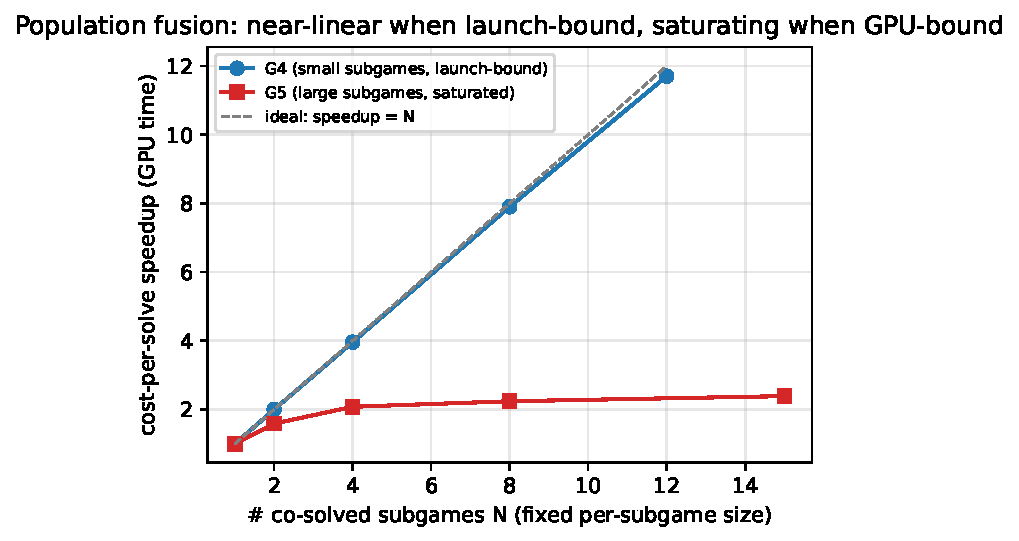
\includegraphics[width=0.78\linewidth]{figs/f1_keysweep.pdf}
\caption{\textbf{The two-regime cost model in one picture.} Cost-per-solve speedup
(GPU-event time, fused vs sequential per-tree GPU-CFR; the sequential arm is bracketed
end-to-end around its per-tree host loop) as a function of the number $N$ of co-solved
subgames (public keys) at fixed per-subgame size. Goofspiel-4 (G4; small subgames, blue)
is launch-bound: fused time is $\sim$constant (197.6 $\to$ 202.4 ms for
$N{:}\,1{\to}12$), so speedup tracks the ideal $\text{speedup}=N$ line (dashed).
Goofspiel-5 (G5; large subgames, red) saturates the device at $N{=}1$: speedup plateaus
at $\sim$2.4$\times$. \emph{How to read the two regimes:} on the blue curve every added
subgame rides along nearly free --- the device was starving --- so the curve hugs the
diagonal until the device fills; on the red curve one subgame already fills the device,
so co-scheduling buys nothing and the residual plateau is launch-overhead recovery only.
Timings are medians of 7 repeats after 3 discarded warmups, with 300 CFR+ iterations.}
\label{fig:keysweep}
\end{figure}

\subsection{End-to-end training win, Goofspiel-4}

Microbenchmark speedups routinely die inside real training loops; this one survives,
because the loop is dominated by exactly the phase we fused. Running the full \S2.2 loop
under the single advance-fixed configuration of \S5, with both arms sharing each of 5
seeds:

\begin{itemize}
\item \textbf{Inner-resolve speedup 11.79$\times$} (median of per-seed ratios; per-seed
range 11.68--12.23) --- against the regime model's launch-bound prediction of
$\sim$11.7$\times$ from the \S6.1 sweep, made before these runs.
\item \textbf{Total wall-clock speedup 9.99$\times$} (per-seed range 9.97--10.41):
median total wall \textbf{fused 76.8 s vs sequential 767.2 s} per arm.
\item \textbf{The Amdahl arithmetic closes ex post.} Write each arm's loop total as
inner plus non-inner time, $T = I + O$, and define per-seed $f =
I_{\text{seq}}/T_{\text{seq}}$ (the inner-resolve fraction) and $S_{\text{inner}} =
I_{\text{seq}}/I_{\text{fus}}$. Exactly,
\[ \frac{T_{\text{seq}}}{T_{\text{fus}}} \;=\; \frac{1}{(1-f) \;+\; f/S_{\text{inner}}
\;+\; \Delta O/T_{\text{seq}}}, \qquad \Delta O = O_{\text{fus}} - O_{\text{seq}}, \]
and since the non-inner phases perform identical work in both arms (\S5), $\Delta O$ can
only be timing noise, leaving the Amdahl ceiling $1/\big((1-f) +
f/S_{\text{inner}}\big)$~\citep{Amdahl1967}. The inner re-solve is \textbf{98.44\%} of
the sequential baseline loop (98.4\% rounded elsewhere); given the measured inner
speedup ($S_{\text{inner}} = 11.79\times$; the ex-ante prediction was 11.7$\times$), the
implied ceiling is \textbf{10.09$\times$} (computed from the unrounded artifact value $f
= 0.9844$; this is the \emph{median}-implied ceiling --- each seed's ratio is bounded by
its own seed-level ceiling, which varies with that seed's $f$ and $S_{\text{inner}}$,
and all five seeds satisfy theirs in the artifacts; a seed's total-wall ratio can exceed
its own implied ceiling only through noise-scale non-inner timing asymmetry, $\Delta O <
0$) --- and the measured 9.99$\times$ sits at 99\% of it. To be precise about what is
prediction and what is accounting: the \emph{microbenchmark predicted the inner-resolve
ratio ex ante} (the microbenchmark runs predate the loop runs; the ordering is
verifiable from the released commit history, Appendix~F); the Amdahl decomposition uses
$f$ measured from the loop itself and is an accounting-consistency closure --- the
residual 1\% reflects the non-inner phases together with the across-seed median
aggregation. The same decomposition, run in reverse, is the contamination diagnostic of
\S6.4.
\item \textbf{Descriptive band check, not improvement.} Fused final NashConv median
\textbf{0.0402} [10th/90th: 0.0238, 0.0533]; sequential median \textbf{0.0469}
[10th/90th: 0.0313, 0.0604, derived from the released per-seed artifacts]. The arms
satisfy the \S5 descriptive band criterion --- each arm's median lies within the other
arm's per-seed 10th/90th interval --- and we make no lower-exploitability claim. The
criterion is a descriptive band check at $n{=}5$, not an equivalence test; equivalence
testing in the two one-sided tests (TOST) style is deferred to the pre-registered
full-protocol G5 run.
\item \textbf{Secondary, threshold-sensitive view (time-to-band).} A time-to-band
$\tau$-sweep ($\tau \in [0.05, 0.12]$) --- where time-to-band($\tau$) is the cumulative
inner-resolve-plus-net-train wall-clock (measurement phase excluded) to the first
measurement round whose on-policy NashConv is $\le \tau$ --- gives speedups from
\textbf{5.5$\times$ to 11.4$\times$} depending on the threshold; at the pooled band
ceiling $\tau = 0.0598$, the median time-to-band is fused 34.7 s vs sequential 190.2 s
(ratio of the per-arm medians, 5.48$\times$; these are time-to-band medians --- the
totals behind the 9.99$\times$ headline are the 76.8/767.2 s above).\footnote{The
non-monotone dip at $\tau = 0.06$ is a quantization artifact of the every-2-rounds
measurement cadence, not a performance effect; the full sweep, the threshold definition,
and the explanation are in Appendix~D.1.} We disclose the full range and keep the
headline on the threshold-free total-wall number, 9.99$\times$.
\item \textbf{Substrate scope (best-vs-best).} The 9.99$\times$ is the same-substrate
fused-vs-sequential comparison that isolates the mechanism (\S4.6). Against the
strongest measured \emph{non-fused} cell in the released bundle --- the same kernel sequential on
the host CPU --- the per-belief 2$\times$2 of \S4.6 puts the G4 best-vs-best win at
$\sim$2.7$\times$ (GPU-fused 0.201 s/belief vs CPU-sequential 0.547 s/belief), pending
matched full-configuration CPU timings (single-run CPU cells; \S4.6,
Appendix~C); the same-substrate tooling question --- the
CUDA-Graphs/\texttt{torch.compile} sequential arm --- is measured in \S6.5. In these
runs, in the launch-bound regime, fusion is what made the GPU the faster substrate at
all.
\item \textbf{Gates.} CPU exact parity $<10^{-9}$; CPU determinism --- fused and
sequential training trajectories identical to all recorded digits (reduced 4$\times$10
budget; \S5); on CUDA, compounding \texttt{index\_add\_} atomics produce per-seed
fused-vs-sequential final-NashConv differences of median 0.0144 (max 0.0389) with no
detectable bias at this seed count (fused higher on 2/5, lower on 3/5; $n{=}5$ is
underpowered to exclude moderate bias, and pooled with the quiet-host G5 pairs the tally
is fused-higher on 4/8) --- the \S5 finding that per-seed equivalence checks of batched
GPU CFR through a training loop will spuriously fail. Mild host sensitivity is visible
even in these clean G4 runs, at much smaller scale than the G5 event (Appendix~B.3).
\end{itemize}

\begin{figure}[t]
\centering
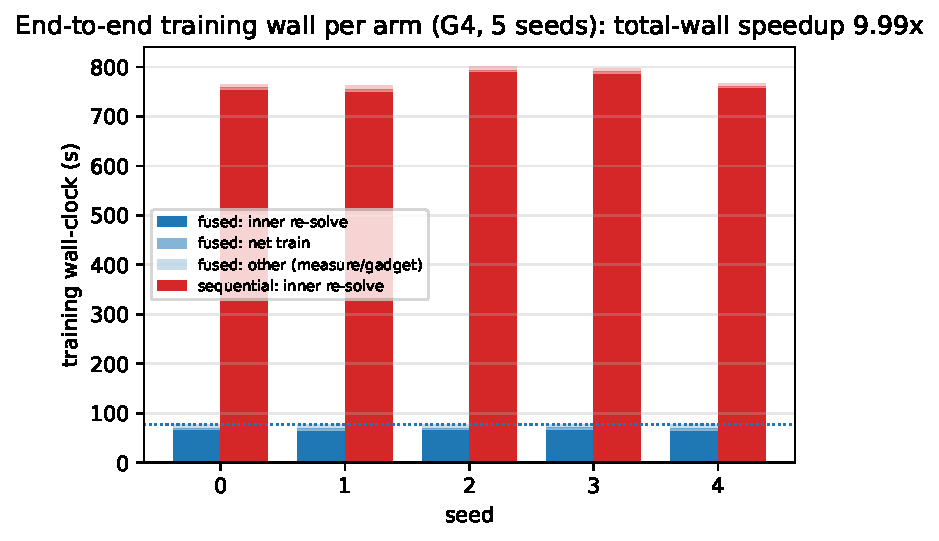
\includegraphics[width=0.85\linewidth]{figs/f2_e2e_wall.pdf}
\caption{\textbf{The end-to-end win, per seed.} Training wall-clock per arm at
Goofspiel-4, stacked by phase (inner re-solve / net train / other, where ``other'' is
the separately-tracked measurement phase; the gadget pass runs after the timed loop and
is outside all phase timers), for all 5 matched seeds. The inner re-solve is 98.4\% of
the sequential arm --- the Amdahl fraction that lets the 11.79$\times$ inner speedup
survive as a 9.99$\times$ total-wall speedup (dotted line: fused median).}
\label{fig:e2ewall}
\end{figure}

\begin{figure}[t]
\centering
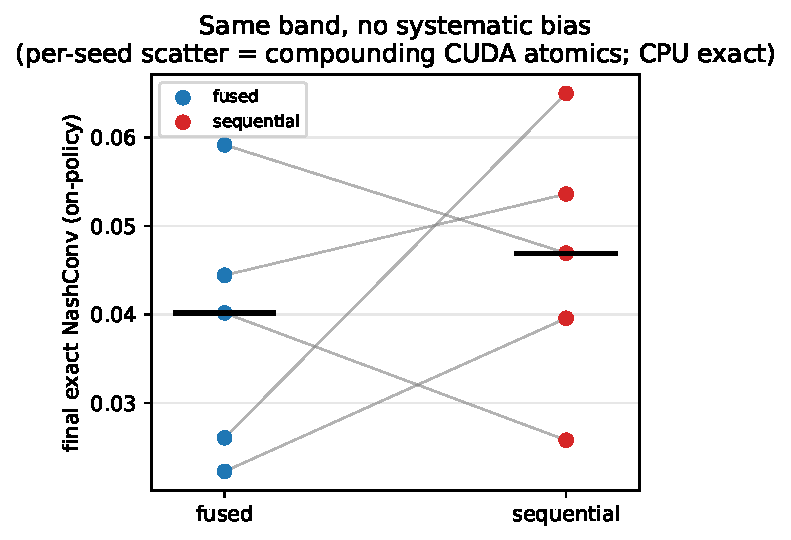
\includegraphics[width=0.7\linewidth]{figs/f3_band.pdf}
\caption{\textbf{Descriptive band check; no detectable bias ($n{=}5$).} Final exact NashConv
(on-policy continuation) of both arms at Goofspiel-4, per seed, with paired per-seed
lines and medians (black bars): fused 0.0402 vs sequential 0.0469. The per-seed scatter
(median $|$diff$|$ 0.0144, max 0.0389; fused higher on 2/5, lower on 3/5) is the
compounding-CUDA-atomics effect of \S5 --- algorithmic equivalence is proven on CPU,
where trajectories are identical to all recorded digits; the seed-sign tally is
consistency evidence, not proof of an unbiased CUDA drift process.}
\label{fig:band}
\end{figure}

\subsection{Search-free boundary (directional only)}

Neural Fictitious Self-Play (NFSP)~\citep{HeinrichSilver2016} learns without any
decision-time or train-time search: it trains a best-response network against an
\emph{average-policy} network that imitates the agent's own historical play, and it is
that averaged policy --- the quantity that converges toward equilibrium --- that we
evaluate (the green curve of Figure~\ref{fig:exploitwall}). To calibrate what the
resolving apparatus buys per unit compute --- not to claim a converged comparison --- we
run NFSP in average-policy mode under one published configuration (\S5; chosen over a
tuned PPO-with-averaging baseline for the reasons given in
Appendix~D.2~\citep{Rudolph2025}). After 600 s ($\sim$640k/629k episodes on seeds 0/1),
NFSP's exact NashConv is \textbf{1.3968 / 1.3966}, barely below the uniform policy's
1.4167; the fused resolving arm reaches its $\sim$0.04 final band in $\sim$77 s total
--- roughly 1/8th of that wall-clock, to a band NFSP has not approached. This is a
\emph{directional boundary only}: NFSP's literature operating point is
$10^6$--$10^7$ episodes, and we report it to locate the resolving loop on the compute
axis, not to rank methods. The accompanying methodology point (detail in Appendix~D.2):
RPG/QPG current-policy NashConv oscillates at $\approx$1.4334 --- \emph{above} uniform
--- so reporting it as the search-free boundary would artificially inflate our
advantage, and we reject it; VRPO is cited as the strongest search-free boundary we are
aware of and deliberately not reimplemented.

\begin{figure}[t]
\centering
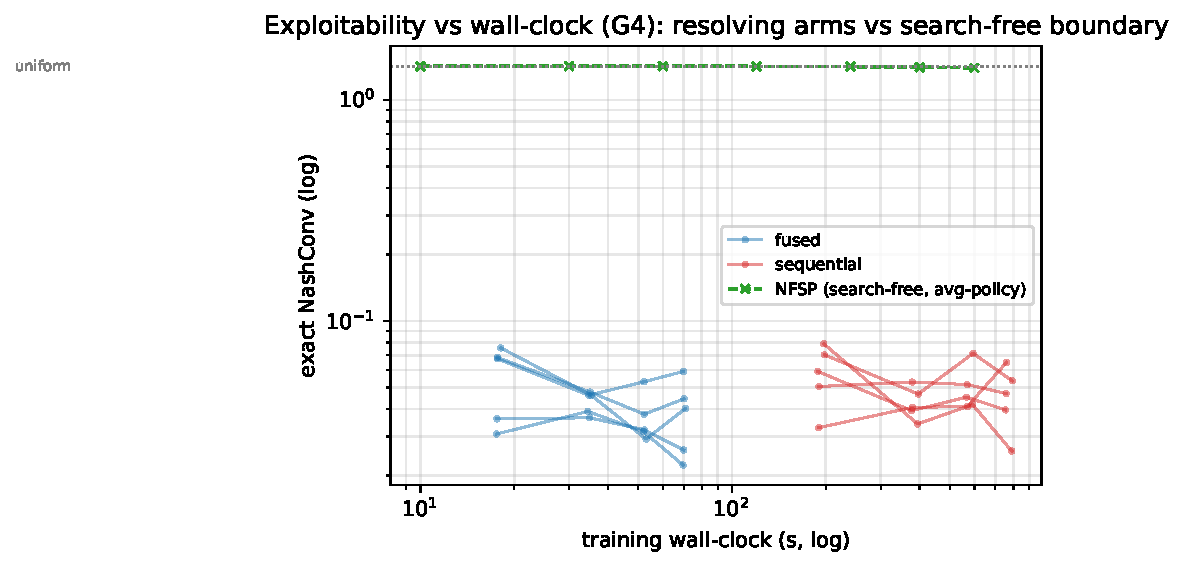
\includegraphics[width=0.78\linewidth]{figs/f4_exploit_vs_wall.pdf}
\caption{\textbf{Exploitability vs wall-clock (Goofspiel-4, log--log).} Exact NashConv
against cumulative training wall-clock: fused arm (blue) and sequential arm (red), 5
seeds each, with the NFSP average-policy curve (green, dashed) and the uniform-policy
level (dotted). Both resolving arms descend to the descriptive band --- fused $\sim$10$\times$
earlier; NFSP remains near uniform for its full 600 s budget (directional boundary
only).}
\label{fig:exploitwall}
\end{figure}

\subsection{Goofspiel-5 at scale: the 5-seed band and the saturated-regime end-to-end point}

\textbf{(a) The 5-seed exploitability band --- a target-construction result.} Scope
first: this result is about what fusion makes \emph{affordable} --- per-belief
finite-budget CFR+ targets at 236k infosets --- and it compares two \emph{target
constructions}; it is \textbf{not} a fused-vs-sequential comparison, and the arms
comparison everywhere in this paper remains equal-band only. The reference point is the
\textbf{0.21 fixed-continuation floor}: in an earlier experiment under the same
implementation and metric (artifacts in the release, Appendix~F), the value net was
trained on targets computed under a \emph{fixed} below-cut continuation policy rather
than per-belief re-solving, and G5 exploitability plateaued at $\approx$0.21 regardless
of additional net training. Why a floor arises: targets computed under one frozen
continuation are \emph{incoherent off-path} --- they answer ``what is this state worth
if play continues in a way that no policy consistent with the belief actually plays''
--- so the value net regresses toward numbers that no assembled policy attains, and the
loop's achievable exploitability is capped by this target incoherence rather than by
optimization effort (a \emph{target-coherence} ceiling; value-error-to-exploitability
propagation in the sense of~\citep{KovarikLisy2019}). Per-belief $V_T$ targets ---
affordable at G5 precisely because the fused solver cuts the cost of the $K{=}15$-key
population re-solve --- remove the incoherence. Under the identical advance-fixed
protocol (\S5 full configuration; 320 resolved beliefs per seed; exact NashConv on the
assembled policy), the five seeds give:

\begin{table}[t]
\centering
\caption{Goofspiel-5 per-belief finite-budget target band (full 8-round protocol, fused path).}
\label{tab:g5band}
\begin{tabular}{cccc}
\toprule
seed & on-policy NashConv & gadget-safe NashConv & final target-net val MAE \\
\midrule
0 & 0.0760 & 0.0880 & 5.8\% \\
1 & 0.1133 & 0.1228 & 6.1\% \\
2 & 0.1282 & 0.1380 & 6.1\% \\
3 & 0.0923 & 0.1010 & 6.0\% \\
4 & 0.1015 & 0.1104 & 6.1\% \\
\bottomrule
\end{tabular}
\end{table}

\begin{itemize}
\item \textbf{On-policy band: median 0.1015 [10th/90th: 0.0825, 0.1222].} Gadget-safe
band: median 0.1104 [10th/90th: 0.0932, 0.1319] --- reported alongside per \S5, with
band claims on the on-policy continuation.
\item \textbf{All 5/5 seeds finish below the 0.21 fixed-continuation floor}; the median
improvement over the floor is \textbf{2.07$\times$}. As delimited above, this is a
target-construction comparison --- what fusion makes affordable --- orthogonal to fusion
itself; it is \textbf{not} a fused-vs-sequential quality claim.
\item The final target-net validation MAE is tight across seeds (5.8--6.1\%), and we find
\textbf{no reproducible improves-with-target-compute trend below $\sim$0.13} (across the
5 band seeds and the earlier seed-0/1 curve runs; Appendix~F) --- initialization and
optimization noise dominate there, which is why this is a band with percentile error
bars and not a curve, and why all speed claims in this paper are equal-band-faster.
\end{itemize}

\textbf{(b) The saturated-regime end-to-end point.} The \S6.1 model predicts that at G5
--- where a single subgame fills the device --- the in-loop inner-resolve speedup should
fall from G4's $\sim$11.7$\times$ to the saturated plateau, microbenchmark value
2.37$\times$. We test this with the same paired-arm design at G5 (shortened budget per
\S5: 4 rounds $\times$ 40 beliefs, single final exact measurement, gadget evaluation
skipped). The headline numbers are the \textbf{quiet-host re-run}: 3 matched seeds
$\times$ both arms on an otherwise idle machine, run after a host-load contamination
diagnosis in the original 2-seed pair (summarized below; full forensics in
Appendix~B.3).

\begin{itemize}
\item \textbf{Inner-resolve speedup 2.40$\times$ (median of per-seed ratios, $n{=}3$,
quiet host; per-seed 2.373/2.400/2.398)} --- within $\sim$1.1\% of the microbenchmark
prediction of 2.37$\times$ (unrounded: 2.398 vs 2.372). Together with \S6.2 (G4:
$\sim$11.7$\times$ predicted $\to$ 11.79$\times$ measured, $n{=}5$), the regime model's
microbenchmark-to-loop transfer holds at both ends.
\item \textbf{The original 2-seed pair is superseded by the quiet-host re-run, but
reported as host-load sensitivity evidence.} The diagnostic
that exposed it: the pair's total-wall ratio (2.20$\times$) \emph{exceeded} the
2.04$\times$ Amdahl ceiling implied by its own measured inner fraction --- by the \S6.2
decomposition this requires a $\Delta O$ an order of magnitude beyond the noise scale
that identical non-inner work can produce. The per-round artifacts located the cause:
host-load-sensitive GPU-event spans in the launch-heavy \emph{sequential} arm (the \S5
timing-discipline mechanism --- the fused arm, issuing $\sim$15$\times$ fewer launch
sequences per belief, stayed fed). The quiet-host $n{=}3$ re-run supersedes the pair ---
prediction 2.37$\times$, measurement 2.40$\times$ --- and restores the self-consistency
check the contaminated pair failed (next bullets). Per-round event spans, the inflation
figures, the contaminated pair's face-value readings, and the $\Delta O$ accounting
applied to it are in Appendix~B.3.
\item The inner re-solve is \textbf{86.1\%} of the sequential loop (median, $n{=}3$,
quiet host; below G4's 98.4\% because the single final measurement is a larger share of
the shortened run).
\item \textbf{Total-wall speedup 2.00$\times$ (median of per-seed ratios; per-seed
1.99/2.00/2.00), against the 2.01$\times$ Amdahl ceiling} implied by the measured
86.1\% inner fraction and the 2.40$\times$ inner ratio --- the accounting now closes to
within 0.3\% (computed from unrounded artifact values, as in \S6.2; the quiet-host
re-run itself realizes one sub-percent per-seed ceiling excess, which the $\Delta O$
reading accommodates), the same closure as G4's, where the contaminated pair had
violated its own ceiling. A time-to-band $\tau$-sweep is flat at 2.39$\times$ across
$\tau \in [0.05, 0.12]$: with a single final measurement, time-to-band coincides with
the training wall-clock, so the G4-style cadence sensitivity (\S6.2) cannot arise here.
\item \textbf{On final exploitability we make a divergence-scale-consistency statement,
not a band claim.} Per-seed finals (fused, sequential): seed 0 \textbf{(0.1543,
0.0912)}, seed 1 \textbf{(0.0974, 0.0857)}, seed 2 \textbf{(0.1243, 0.1457)}. The fused
final is higher (worse) on \textbf{2/3} seeds --- a direction $n{=}3$ cannot assess,
which we state rather than imply away. The per-seed divergences (0.0631/0.0117/0.0214)
are consistent in scale with the compounding-CUDA-atomics envelope documented at G4
(median 0.0144, max 0.0389; the G5 max exceeds it $\sim$1.6$\times$) --- not
inconsistent with the \S5 mechanism, though the envelope's scaling with game depth is
uncharacterized, which the planned full-protocol G5 run will bound. These
shortened-protocol (4-round) finals are \emph{not comparable} to the 8-round 5-seed band
above in either direction, and two of the six lie outside that band's observed range ---
so no band-membership claim is available from these runs, and we make none.
Through-training equivalence at G5 rests on the CPU gates and the single-solve parity
($4\times10^{-6}$); establishing statistical CUDA non-divergence at G5 requires the planned
full-protocol $n \ge 5$ paired run with a pre-registered margin. No lower-exploitability
claim is made in either direction.
\item The safe-resolving gadget is outside all timing claims: it runs after the timed
loop, outside every phase timer and outside \texttt{total\_wall} (\S5). The quiet-host
paired G5 runs skip it uniformly; placement notes and the superseded pair's single
post-loop gadget reading are in Appendix~D.4.
\end{itemize}

The two G5 results compose into the paper's working point: the fused solver makes
per-belief finite-budget CFR+ targets affordable at 236k infosets (the band above), and even in
the regime where fusion pays \emph{least}, it still pays the predicted $\sim$2.4$\times$
on this device --- with the prediction made by a model fit on microbenchmarks alone.

\subsection{Launch-amortization ablation: the headline comparison under tool symmetry}

\S4.6 identified CUDA-Graphs capture and \texttt{torch.compile(mode="reduce-overhead")}
as the rival lever and promised the measured ablation; here it is, in both directions.
Six arms --- \{fused, sequential\} $\times$ \{eager dispatch, compiled, graph-captured\}
--- on the \S6.1 protocol (300 CFR+ iterations, median of 7 repeats after 3 discarded
warmups, float64, precompiled topologies; compile/capture setup walls excluded
symmetrically and reported in the artifact: \texttt{torch.compile} $\le$9.3 s per game,
graph capture $\le$0.15 s). The graph-captured arms replay an even/odd CUDA-Graph pair
executing the \emph{same} kernel sequence as eager --- pure launch amortization ---
while the compiled arms additionally re-codegen (fuse) the per-iteration kernels; the
two tools therefore separate launch overhead from eager-ATen kernel inefficiency
(capture engineering in Appendix~C.1). Parity is gated as everywhere: at per-tree
granularity the tooled sequential arms match the eager reference to
$\le 3.3\times10^{-11}$ at G3/G4 (gate $10^{-9}$); at fused granularity G3/G4 pass with
over 2.5 orders of margin (compile $3.0\times10^{-12}$, graphs $5.4\times10^{-14}$ at
G4, against an eager-rerun atomics floor of $1.4\times10^{-12}$); at G5 the gate is
\textbf{floor-limited}: the eager fused reference differs from \emph{itself} by
$\sim$$2\times10^{-8}$ between reruns (CUDA \texttt{index\_add\_} atomics over $B{=}125$
cut nodes $\times$ 236k infosets compounded through the 200-iteration parity run;
reproduced at $5.7\times10^{-9}$--$1.7\times10^{-8}$ across independent rerun pairs),
and the tooled arms sit at 1.00--1.05$\times$ that floor --- indistinguishable from an
eager rerun, with no evidence of a numerics change, but not certifiable to $10^{-9}$. G5
rows below carry this caveat.

\textbf{Step 1 --- the asymmetric comparison (the natural first comparison).}
Amortize the \emph{sequential} arm only, and compare it against the eager-dispatched
fused solver. Launch amortization is real: it lowers the sequential per-tree floor by
72\%/66\% (compile/graphs) at G4 and 63\%/32\% at G5. But the amortized sequential arm
\emph{remains linear in $N$} (G4 compile slope 56.82 ms/tree, vs 201.09 eager) while the
eager fused arm stays flat, so the fused advantage is rescaled, not removed: the
surviving best-vs-best speedups are \textbf{2.59$\times$ (G3), 3.28$\times$ (G4),
1.03$\times$ (G5)}, with the G4 crossover moving from $N^*\!\approx\!1$ to
$N^*\!\approx\!3.63$ and the retained advantage still growing as $\sim N/3.63$. The G5
reading decomposes exactly as \S4.6 predicted for capture --- pure graphs recover only
1.31$\times$ of the sequential arm's cost and the eager fused arm retains 1.85$\times$
over them --- but \texttt{torch.compile} goes further: its within-tree kernel re-codegen
brings the compiled \emph{sequential} arm to parity with the eager-ATen \emph{fused} arm
(1.03$\times$). Taken alone, this table understates the mechanism, because it grants
amortization tooling to one arm and not the other; we report it because it is the
comparison this setup produces first, and because the asymmetry is exactly what
motivates step 2.

\textbf{Step 2 --- the symmetric comparison (best tool per arm).} The identical tooling
applies to the fused topology unchanged --- the same even/odd-pair and compiled-step
machinery at population granularity --- and the arms then coincide at $N{=}1$ by
construction (G4: 55.2 vs 56.6 ms; G5: 109.6 vs 111.1 ms), so everything beyond $N{=}1$
is the fusion mechanism itself (Table~\ref{tab:sixarm}).

\begin{table}[t]
\centering
\caption{Six-arm launch-amortization ablation (full cut population, 300 CFR+
iterations; ms, GPU-event medians; best amortized arm per side in bold).}
\label{tab:sixarm}
\begin{tabular}{lccccccc}
\toprule
 & \multicolumn{3}{c}{fused} & \multicolumn{3}{c}{sequential} & amortized \\
\cmidrule(lr){2-4} \cmidrule(lr){5-7}
game & eager & compile & graphs & eager & compile & graphs & best-vs-best \\
\midrule
G3 ($N{=}9$) & 117.1 & \textbf{39.1} & 40.0 & 1,059.4 & 355.5 & \textbf{311.7} & \textbf{7.96$\times$} \\
G4 ($N{=}12$) & 202.1 & \textbf{56.6} & 85.5 & 2,426.7 & \textbf{683.0} & 810.2 & \textbf{12.06$\times$} \\
G5 ($N{=}15$) & 1,871.0 & \textbf{1,060.3} & 1,817.4 & 4,536.2 & \textbf{1,929.2} & 3,465.6 & \textbf{1.82$\times$} \\
\bottomrule
\end{tabular}
\end{table}

The sequential arms and eager-vs-eager reference come from the per-key session; the
amortized fused arms were measured in an independent session with the fused-eager arm
re-measured as the cross-session drift anchor (ratios 0.969--0.998). The independent
session is $\le$3\% faster, so the best-vs-best ratios carry $\le$3\% cross-session
uncertainty in fusion's favor; no conclusion is within that margin except the $N{=}1$
coincidence, which holds by construction. The ablation's own eager-vs-eager column
(8.82/11.64/2.42$\times$) reproduces Table~\ref{tab:bakeoff}
(8.77/11.69/2.37$\times$) within $\sim$2\%.

\begin{itemize}
\item \textbf{Launch-bound regime (G4): the fusion advantage is $\text{speedup} \approx
N$, with or without tooling.} The amortized G4 key sweep gives amortized-fused over
amortized-sequential \textbf{1.02/1.97/3.97/7.84/11.62$\times$ at $N = 1/2/4/8/12$} ---
speedup $\approx N$ at every point, the same shape as the eager-vs-eager sweep of
\S6.1. The amortized fused arm is flat (55.2 $\to$ 58.7 ms for $N{:}\,1{\to}12$ ---
slope 0.31 ms/tree on a 55.2 ms floor, +6.2\% for 12$\times$ the population) while the
amortized sequential arm stays linear, and step 1's $N^*\!\approx\!3.63$ crossover
collapses back to $\approx$1. The two levers compose multiplicatively: compile is worth
3.57$\times$ on the fused arm at G4, on top of fusion's $\approx N$ over sequential.
\item \textbf{Saturated regime (G5): step 1's parity verdict reverses to 1.82$\times$.}
Pure capture buys essentially nothing on the fused arm (fused-graphs 1.03$\times$ over
fused-eager): the fused G5 solve is genuinely compute/occupancy-bound, confirming the
\S6.1 saturation story. Compile's kernel re-codegen still buys 1.76$\times$, and under
compile-vs-compile the \emph{marginal} cost per additional tree is 68.0 ms/tree fused
vs 129.6 ms/tree sequential --- so the amortized-vs-amortized speedup rises
monotonically (1.01/1.34/1.60/1.71/1.81$\times$ at $N = 1/2/4/8/15$; 1.82$\times$ on
the cross-game row) toward the marginal-slope ratio $\approx$1.9, with no crossover:
dominance from $N{=}1$. Step 1's G5 parity was an artifact of comparing eager-ATen
fused kernels against compiled sequential ones.
\item \textbf{Regime-model upgrade.} With per-arm floors and slopes, the \S6.1 envelope
refines to $\text{speedup}(N) \approx \big(\text{floor} +
\text{slope}_{\text{seq}}(N{-}1)\big) / \big(\text{floor} +
\text{slope}_{\text{fused}}(N{-}1)\big)$, with $\text{floor}_{\text{fused}} \approx
\text{floor}_{\text{seq}}$ under the same tooling: $\to N$ when
$\text{slope}_{\text{fused}} \approx 0$ (launch-bound; measured 11.62$\times$ at
$N{=}12$), $\to \text{slope}_{\text{seq}}/\text{slope}_{\text{fused}} = 129.6/68.0
\approx 1.9$ at saturation (measured 1.81$\times$ at $N{=}15$). Launch amortization
rescales both arms' floors equally; it cannot touch the cross-tree occupancy term. The
fusion advantage \emph{is} the marginal-cost ratio, and it survives.
\item \textbf{Tool-symmetric end-to-end check (G4).} We reran the full G4 loop with
\texttt{torch.compile} on both arms using 5 matched seeds and the same aggregation
discipline as \S6.2. Fused and sequential pass the same broad descriptive band check
(pooled ceiling $\tau=0.0506$; final medians 0.0475 fused vs 0.0304 sequential; fused
reaches the pooled-ceiling band in 11.0 s train wall, sequential in 109.9 s), and the fused arm is
faster by 11.36$\times$ on inner resolve, 7.38$\times$ on total wall, and
9.99$\times$ time-to-band against a 7.39$\times$ Amdahl ceiling for total-wall speedup.
This is a timing result under a coarse quality gate, not a lower-exploitability result.
The remaining tool-symmetric end-to-end extension is the analogous G5/production-scale
paired CUDA band run.
\end{itemize}

\section{Related Work}

We position the lever inside the cost identity of Eq.~(\ref{eq:cost}), then delimit it
from the nearest structural neighbors. Non-claim-bearing expansions are in Appendix~E.

\textbf{The lever taxonomy of Eq.~(\ref{eq:cost}).} The wall-clock cost of train-time
iterated resolving factors as (number of solves) $\times$ (iterations per solve)
$\times$ (wall-clock per CFR iteration of a solve), with sampling variance per traversal
a further axis when traversals are stochastic. Prior work attacks the first two factors
and the sampling axis; to our knowledge no published work claims the
\textbf{cost-per-solve} factor for \emph{populations} of subgames --- the lever this
paper isolates.

\begin{itemize}
\item \textbf{Number of solves ($N_{\text{solves}}$).} TurboReBeL~\citep{TurboReBeL} is
the nearest cost-efficiency cousin of this paper: it reports matching ReBeL's
exploitability at a small fraction of its training cost by amortizing target generation
across CFR iterations --- its primary lever is \textbf{single-sample multi-iteration
generation} (one sampling pass yields data for all $T$ iterations), with suit/chip
isomorphism augmentation as a secondary, poker-specific lever. It reduces the number of
solve/sampling passes per training datum; each solve is still executed one subgame at a
time. The levers compose: theirs is per-datum solve count, ours is per-solve cost.
\item \textbf{Iterations per solve.} DCFR~\citep{BrownSandholm2019} and
PCFR+~\citep{Farina2021} accelerate the convergence of a single solve by discounting and
prediction. Meta-learned predictive regret minimization --- originated
in~\citep{Sychrovsky2024} and extended to self-play in~\citep{NPCFR} --- trains over a
\emph{distribution} of subgames but deploys on each subgame \emph{sequentially}: it
reduces iterations per solve, not the cost of an iteration, and stacks with our lever.
Deep-Predictive DCFR~\citep{DeepPredictiveDCFR} --- building on Deep
CFR~\citep{Brown2019DeepCFR}, the canonical neural CFR --- and AlphaEvolve-discovered
CFR variants~\citep{AlphaEvolve-CFR} extend this line (Appendix~E).
\item \textbf{Samples per traversal.} MCCFR~\citep{Lanctot2009} and its
variance-reduced descendants VR-MCCFR~\citep{Schmid2019}, ESCHER~\citep{McAleer2023},
and DREAM~\citep{Steinberger2020} reduce the variance (hence the count) of sampled
traversals; the per-iteration arithmetic of each solve is untouched.
\item \textbf{Subgame size.} LAMIR~\citep{LAMIR} learns abstractions that limit each
resolved subgame to a manageable size, making principled look-ahead tractable in games
where it previously could not scale. Smaller subgames \emph{deepen} the launch-bound
regime in which fusion pays most (regime model, \S6.1).
\item \textbf{Cost per solve (this work).} Fusing the population of same-topology
depth-limited PBS subgames generated by one resolving sweep into shared batched kernel
launches, with parity to per-tree CFR+ gated as in \S5.
\end{itemize}

\textbf{GPU-accelerated CFR.} Kim~\citep{Kim2024} vectorizes CFR \emph{within} a single
game tree, reporting speedups of up to 401.2$\times$ over OpenSpiel's Python CFR and up
to 203.6$\times$ over its C++ implementation; our sequential baseline arm has exactly
this shape (the same level-grouped
SoA kernel, applied one subgame at a time). Kim \& Sandholm~\citep{KimSandholm2026}
reframe CFR as a series of linear-algebra operations --- a
sequence-form-as-linear-algebra formalization with proven work--depth bounds for the
parallelized iteration (total work $W = \Theta(|P|)$ at depth $D = \Theta(k \log B)$, in
their notation) and measured speedups of up to four orders of magnitude over OpenSpiel's
CPU implementations --- and the authors' NoRegret library
(v0.0.0.dev15, released 2026-06-04) makes this an actively developed, still per-tree
line; a GPU-CFR implementation for the card game Pasur~\citep{Pasur-GPU} and the
open-source gpucfr code (CTU Prague)~\citep{gpucfr} are further per-tree/per-game data
points. Li and Huang's Real-Time Parallel CFR~\citep{RealTimeParallelCFR} is the newest
adjacent HUNL systems result we found: it parallelizes a single depth-limited CFR solve
through CPU/GPU pipeline stages, pruning, abstraction, and GPU leaf evaluation. That is
orthogonal to the lever isolated here, which fuses a population of same-topology solves
generated by one resolving sweep into shared kernel launches. As of 2026-06-11 we find
no public work claiming population-level fusion on this line. We note plainly that in the linear-algebra
formulation of~\citep{KimSandholm2026}, a \emph{mechanical} multi-tree batch dimension
is an anticipatable engineering extension --- a block-diagonal arrangement NoRegret
could ship in a point release. What this paper claims is therefore the conjunction, not
the batch dimension: the identification that \emph{iterated resolving structurally
generates} the population, the parity-gated loop integration with shared range-vector
state, and the predictive regime model with its end-to-end validation. Those survive
even if per-tree libraries add batching.

\textbf{Batched solving and adjacent claims in game solving.} Six nearby claims are
distinct from ours. (i) Marris et al.~\citep{Marris2022} batch equilibrium solving, but
with a \emph{learned, amortized} solver over \emph{normal-form payoff matrices}; we run
parity-gated CFR+ over \emph{extensive-form} depth-limited PBS subgames --- variable
depth, chance nodes, per-subgame regret and range state --- inside a training loop.
(ii) DeepStack's batching is net-eval batching, not solve batching. (iii) The
distribution-of-subgames in~\citep{NPCFR} is a meta-training set for a predictor that is
then applied sequentially per subgame. (iv) US Patent
11,204,803~\citep{USPTO11204803} decomposes the game into independently solvable
subtasks --- task-level parallelism, not fusion of many solves into shared kernel
launches on one device. (v) The within-public-state range dimension --- solving for all
private hands simultaneously --- is classical~\citep{Johanson2011,Johanson2012} and is
present in \emph{both} of our timing arms; our claim is the across-key axis (\S2.2,
\S4.5). (vi) Concurrent subgame solving per se has distributed-CPU precedent: Cepheus,
which essentially solved heads-up limit hold'em, decomposed the game into a trunk and
subgames solved concurrently across distributed CPU
nodes~\citep{Bowling2015,Tammelin2015}; what is unclaimed is the single-device
GEMM-fusion of the subgame population into one kernel-launch sequence.

\textbf{Continual resolving and decision-time search.} DeepStack~\citep{Moravcik2017}
introduced continual resolving with neural counterfactual-value leaves; what it batches
are \emph{net evaluations} at subgame leaves, not the solves themselves. Naive
depth-limited solving is unsound~\citep{BrownSandholm2018}; safe-resolving
gadgets~\citep{Burch2014,Moravcik2016,Moravcik2017} and safe-and-nested subgame
solving~\citep{BrownSandholm2017} restore soundness (the background is carried by
\S2.2). ReBeL~\citep{Brown2020} moved resolving into the training loop on public belief
states --- the loop whose inner solve we fuse --- and Student of
Games~\citep{Schmid2023} unified search-based agents across game classes; within this
line, TurboReBeL and LAMIR attack $N_{\text{solves}}$ and subgame size respectively
(taxonomy above). Kubicek, Lisy \& Sandholm~\citep{Kubicek2026} show that
resolving-gadget equilibria are non-unique and refinement-sensitive; accordingly, our
exploitability-band claims use the on-policy re-solve continuation, with gadget numbers
reported alongside (\S5). The agent lineage (Libratus, Pluribus) and opponent-model
resolving (CDBR) are discussed in Appendix~E.

\textbf{Systems prior art: batching small workloads.} The batching economics themselves
are classical and we do not claim them: \S2.3 reviews the batched-BLAS insight and the
roofline frame, and the FlashAttention template we follow is credited in \S1. CUDA
Graphs~\citep{CUDAGraphs} amortize launch overhead for a fixed kernel sequence without
fusing work --- the rival lever, analyzed for our kernel in \S4.6. In the games-adjacent
systems literature, mctx~\citep{Danihelka2022} batches MCTS search populations in the
perfect-information family; Pgx~\citep{Koyamada2023}, EnvPool~\citep{Weng2022}, and
Isaac Gym~\citep{Makoviychuk2021} vectorize game/environment \emph{simulation}, not
iterative coupled-state solving (distinctions in Appendix~E). None of these carries a
shared cross-instance regret table through a clamped fixed-point solve under an
exactness gate --- that conjunction, in the extensive-form resolving loop, is what is
new here; the batching pattern itself is not, and we do not claim it.

\textbf{Search-free self-play.} NFSP~\citep{HeinrichSilver2016} and regret/Q-based
policy gradients (RPG/QPG)~\citep{Srinivasan2018} learn without decision-time search;
our directional search-free boundary uses NFSP's \emph{average} policy, since evaluating
the RPG/QPG \emph{current} policy early in training is near-uniform and would be a weak
comparison (\S6.3, Appendix~D.2). VRPO~\citep{VRPO} reports a positive win rate against
Slumbot in HUNL --- a result its authors describe as
not a decisive win --- without online search or subgame solving, and is the strongest
search-free line we are aware of; we cite rather than reimplement it, because the
primary baseline for a cost-per-solve claim is the in-experiment sequential arm
sharing the same kernel, the same seeds, and gated parity.

\section{Limitations, Scope, and Future Work}

\textbf{Scope of the demonstrated loop.} Our end-to-end demonstration is a
\textbf{2-level, single-cut} iterated-resolving loop: the trunk is re-solved against
value targets obtained by re-solving each cut subgame at sampled beliefs, and these
per-belief targets are \emph{independent given the belief}. This independence is exactly
what makes the population of subgames fusable, so the obvious objection --- surfaced at
the end of \S4 --- must be answered plainly: \emph{is this just batching embarrassingly
parallel work?} Our rebuttal is a conjunction, and we do not claim any single ingredient
is novel in isolation: (a) identifying that train-time iterated resolving
\emph{structurally generates} a population of same-topology depth-limited PBS subgames
--- a common and important target-generation workload in this lineage (DeepStack's
$10^7$ independently re-solved subgames, \S2.2); (b) a fused CFR+
whose nontrivial content is the level-grouped compilation of irregular structure,
float64 discipline through compounding fixed-point iterations, and live-loop
integration, with parity to the sequential solver gated rather than assumed (\S4.5 ---
the within-key coupled state is classical~\citep{Johanson2011,Johanson2012} and not the
novelty); (c) a predictive floor/slope regime model,
$C_{\rm seq}=a_s+b_s(N-1)$ and $C_{\rm fus}=a_f+b_f(N-1)$, with the
$\min(N,1/\varphi)$ expression retained as the launch-bound envelope and with an
operationalized two-point marginal-cost probe (\S6.1); and (d) an Amdahl-surviving
end-to-end result (the ex-ante inner
prediction 11.7$\times$ realized at 11.79$\times$; total-wall accounting closing to
within 1\% of the 10.09$\times$ ceiling). A relevant structural distinction for what
lies beyond: DeepStack-style \emph{independent target generation} is fully fusable,
while ReBeL-style \emph{episodic} resolving is serially coupled along an episode
(fusable across parallel episodes and keys, not along the chain); and the belief axis is
a second fusion dimension --- our loop already solves 40 sampled beliefs per round as 40
separate fused solves over a belief-independent topology, so beliefs can be folded into
the population to restore the fused width when level-coupling shrinks $K$. The strongest
form of the claim --- fused-vs-sequential \textbf{timing under $\geq$3-level nested
resolving}, where targets become serially coupled across levels --- is deferred to
future work. Multi-level self-play \emph{correctness} on this implementation is already
certified (Goofspiel-4: exploitability decreases 0.0506 $\to$ 0.0145 with training;
recorded in the supplementary measurement notes, Appendix~F; a standalone artifact is
planned); only the multi-level timing comparison is outstanding.

\textbf{Baseline tooling and substrate.} The \S6.2/\S6.4 end-to-end speedups are
measured against an eager-dispatch, single-stream sequential arm. The
CUDA-Graphs/\texttt{torch.compile} tooling question is now measured at the
cost-per-solve level, in both directions (\S6.5, Appendix~C.1): under tool symmetry
fusion retains $\text{speedup} \approx N$ launch-bound (12.06$\times$ at G4) and
$\sim$1.8$\times$ at saturation. The G4 tool-symmetric end-to-end check is now complete:
compiled-vs-compiled fusion gives 11.36$\times$ inner and 7.38$\times$ total-wall
speedup while passing the same broad descriptive band check (final medians 0.0475 fused
vs 0.0304 sequential). The remaining item on this axis is the analogous
G5/production-scale paired run. Our own CPU-gate artifacts imply that
at G4 scale the GPU-sequential arm is $\sim$4.3$\times$ slower per belief than the same
kernel on the host CPU --- making the cross-substrate best-vs-best G4 win
$\sim$2.7$\times$ as currently measurable (single-run CPU cells, no timing discipline;
\S4.6, Appendix~C); matched full-configuration CPU timings (G4 and G5) remain planned.
Multi-stream per-tree dispatch and fp32-with-compensated-accumulation are further
untested alternatives in the same family.

\textbf{One game family, one device.} All end-to-end timing is on the Goofspiel ladder;
Leduc and liar's-dice are parity-tested for the fused solver but not end-to-end timed.
All measurements use a single consumer GPU (RTX 3070 Ti, 8 GB) whose FP64 throughput is
1:64 of FP32 --- an extreme placement for a float64 workload. The regime model is
likewise subject to memory capacity (\S6.1): the 8 GB card bounds the fusable population
($B_{\max}$ unmeasured; every population in this paper fits), and peak VRAM per arm is
not yet instrumented. The direction of this asymmetry is \emph{favorable} to the lever:
on a data-center
part with 1:2 FP64 (A100) and $\sim$10$\times$ the FP64 throughput, both the effective
launch floor and the saturation point would change; the model predicts the outcome only
after measuring the regime probe on that device. On this device, the both-ends
validation and the HUNL-mass argument below hold as measured; their numeric values are
device-conditional, and A100 replication is future work.

\textbf{Exploitability is a band, not a curve.} On the largest instance (Goofspiel-5,
236,450 infosets) final exploitability sits in a 0.07--0.13 band where initialization
and optimization noise dominate (below $\sim$0.13 we found no reproducible
improves-with-target-compute trend). We therefore make \textbf{time-based, equal-band
claims only} --- never lower-exploitability claims --- with both arms sharing seeds. The
completed 5-seed G5 band is on-policy median 0.1015 [10th/90th: 0.0825, 0.1222]
(gadget-safe median 0.1104 [0.0932, 0.1319]; all 5/5 below the 0.21 fixed-continuation
floor, defined in \S6.4). The G5 paired end-to-end finals are shortened-protocol values
that are not band-comparable and have fused higher on 2/3 seeds (quiet-host re-run); per
\S6.4 we make a divergence-scale-consistency statement there, not a band claim.
Fused-vs-sequential equivalence is proven on CPU (exact parity $<10^{-9}$; determinism
identical to all recorded digits at the reduced gate budget); on CUDA,
\texttt{index\_add\_} atomics compound through training into per-seed
final-exploitability differences of median 0.0144 (max 0.0389) at G4 with no detectable
bias at $n{=}5$ (\S5); the divergence envelope's scaling with game depth is
uncharacterized --- the G5 max divergence exceeds the G4 max (\S6.4) --- and the planned
full-protocol G5 run will bound it. Gadget-based safe-resolving numbers additionally
inherit refinement-choice sensitivity~\citep{Kubicek2026}.

\textbf{The saturated regime is a bound, and we state it as one.} When a single subgame
occupies the device, fusion degrades to $\sim$2.4$\times$ on this device (Goofspiel-5:
microbenchmark 2.37$\times$, measured in the end-to-end loop at 2.40$\times$, $n{=}3$
quiet host, \S6.4). We regard this as a \emph{contribution} --- the cost model predicts
where the lever pays (the launch-bound, many-small-subgames regime that iterated
resolving structurally generates) and where it does not --- but it caps the claim: the
$\sim$10$\times$ figure is regime-conditional, not universal. The measured inner
fractions are likewise operating-point properties: the 98.4\% (G4) and 86.1\% (G5)
inner shares reflect a small value network (MLP, hidden 128) and a sparse measurement
cadence; with production-scale value networks the non-inner share grows, $f$ drops, and
the total-wall multiple contracts toward the inner-resolve ratio applied to a smaller
fraction --- exactly as the Amdahl decomposition of \S6.2 prescribes, and in the
direction the G5 point already shows ($f = 86.1\%$ gives a 2.01$\times$ ceiling).

\textbf{Subgame-build ceiling.} The fused \emph{solver} scales ($\approx$6.2 ms/iter
in-loop at Goofspiel-5), but our eager full-enumeration subgame \emph{build} does not:
Goofspiel-6 build exceeds 280 s, capping the demonstrated ladder at $\sim$236k infosets
--- short of the $10^6$--$10^7$ infosets of the large games evaluated
in~\citep{Rudolph2025}. Lazy/direct-SoA construction is future work, not a solver
limitation. Our scope discipline here matches the one Kim \&
Sandholm~\citep{KimSandholm2026} state for
their own technique --- parallelization ``does not necessarily increase the size of the
game that can be solved'': population fusion likewise raises throughput, not maximum
instance size.

\textbf{Future work.} (1) The $\geq$3-level fused-vs-sequential timing demonstration.
(2) The remaining baseline items: matched CPU timings, and the analogous
G5/production-scale amortized-fused vs amortized-sequential end-to-end comparison; the
quiet-host G5 timing re-run is complete ($n{=}3$, \S6.4), and what remains on that axis
is the full-protocol (8-round) $n \ge 5$ paired run with a pre-registered band margin
for a CUDA non-divergence test. (3) A second game family timed end-to-end. (4) A100
replication and multi-GPU sharding --- the population axis shards trivially across
devices (unlike a single tree), so multi-GPU \emph{extends} the lever rather than
competing with it. (5) A HUNL-scale instance built on lazy subgame construction, where
held-out Slumbot~\citep{Jackson2013} becomes the transfer validation; consistent with
our protocol, Slumbot supplies no training data, targets, or selection signal at any
point. A preliminary HUNL topology census suggests many same-topology river classes,
but class size only upper-bounds train-time co-occurrence and the timing probe uses
synthetic payoffs; HUNL timing and held-out Slumbot transfer are future work (mechanics
in Appendix~D.3). (6) Composition with the other
levers of Eq.~(\ref{eq:cost}): pairing the population axis with TurboReBeL-style
$N_{\text{solves}}$ reduction, DCFR/PCFR+/meta-learned iteration reduction, or
MCCFR-family variance levers is untested --- including the interaction risk that
predictive or meta-learned minimizers change the per-iteration op mix the compiled
kernel assumes. The within-loop sequential arm --- the same kernel run
per-tree~\citep{Kim2024} --- remains the primary baseline in every experiment.

\section{Conclusion}

Train-time iterated resolving structurally generates populations of same-topology
depth-limited PBS subgames, and \textbf{population fusion} --- compiling each population
into one level-grouped SoA CFR+ --- isolates across-solve amortization of
the cost-per-solve factor of its cost identity --- wall-clock per solve-iteration,
hence, at the common iteration budget $T$, per-solve wall-clock --- with parity to
per-tree solving verified in float64 and, on CPU, trajectory-identical to all recorded
digits. The claim is deliberately narrow: \emph{equal-band-faster} at G4 under a broad
descriptive band check, same-substrate
against the same kernel run per tree, in a regime the cost model identifies and a
two-point marginal-cost probe classifies --- near-linear in the number of co-solved subgames
while solves are launch-bound (Goofspiel-4: inner 11.79$\times$ predicted ex ante at
11.7$\times$; total wall 9.99$\times$ against a 10.09$\times$ Amdahl ceiling, 5 matched
seeds; under tool symmetry, 11.36$\times$ inner and 7.38$\times$ total wall against a
7.39$\times$ Amdahl ceiling), saturating at $\sim$2.4$\times$ when one subgame fills the device (Goofspiel-5:
2.37$\times$ predicted, 2.40$\times$ measured, 3 matched quiet-host seeds; the
statistical CUDA non-divergence test remains pending). The measured launch-amortization
ablation shows the per-solve advantage survives CUDA-Graphs/\texttt{torch.compile} tool
symmetry --- $\text{speedup} \approx N$ launch-bound (12.06$\times$ at G4) and
1.82$\times$ at saturation (\S6.5). We claim no exploitability improvement,
no cross-substrate superiority beyond the $\sim$2.7$\times$ best-vs-best our artifacts
currently support at G4 (single-run CPU cells; \S4.6), and no generality beyond one game
family and one device until the remaining planned runs --- matched CPU timings, the
G5/production-scale amortized paired run, and multi-device replication --- are complete.
What we
believe travels regardless: the population-fusion lever and its regime model, the
matched-seed paired-arm + CPU-exactness-gate evaluation template, and the warning that
compounding CUDA atomics make naive per-seed equivalence checks of batched GPU CFR
spuriously fail.

\section{Reproducibility Statement}

\textbf{Code, commits, and artifacts.} All experiments live in one repository (release
accompanies the preprint). The evidence-bearing commits: \texttt{c47cc19} --- the
cost-per-solve microbenchmark and controlled key sweep (produces
\texttt{costpersolve\_bakeoff.json}); \texttt{8def574} --- the G4 end-to-end paired arms
and the NFSP search-free boundary; \texttt{1ff6a8e} --- the G5 per-belief target band,
seeds 0--1; and the final-data runs (post \texttt{dd3d148}; release commit pinned at
submission) --- the G5 band seeds 2--4, the original and quiet-host G5 paired end-to-end
runs, the HUNL topology census probe, and the six-arm launch-amortization ablation of
\S6.5 (produces \texttt{cuda\_graphs\_ablation.json}), plus the G4 tool-symmetric
end-to-end check (produces \texttt{e2e\_amortized\_g4\_compile\_summary.json}). Every
JSON cited in this paper is copied into
the tracked directory \textbf{\texttt{release/v1-artifacts/}} with a \texttt{README.md}
manifest and per-file SHA-256 sums; those files are the reproducibility bundle that
accompanies the paper. One-command reproduction lines for
every experiment, the seeds inventory and no-sweep statement, the aggregation
restatement, the artifact field-naming notes, the supplementary-measurement-notes
inventory, and the hardware/software stack with total-compute accounting are in
Appendix~F. The play-time evaluation harness under development for the HUNL-scale
instance of \S8 --- outside this paper's claims --- uses PokerKit~\citep{PokerKit} as
its game-state engine.

\textbf{Held-out integrity.} No Slumbot (or any external-agent) data, targets, priors,
or selection signals are used anywhere in this paper
(\texttt{uses\_slumbot\_data=false}). The HUNL topology census probe (\S8) uses only the
public betting-tree structure under our own abstraction and synthetic shape-faithful
payoff matrices for timing --- no Slumbot interaction of any kind.
\begin{thebibliography}{99}

\bibitem{Abdelfattah2016} A. Abdelfattah, A. Haidar, S. Tomov, J. Dongarra. Performance,
Design, and Autotuning of Batched GEMM for GPUs. \emph{ISC High Performance} 2016.

\bibitem{Abdelfattah2021} A. Abdelfattah, T. Costa, J. Dongarra, et al. A Set of Batched
Basic Linear Algebra Subprograms and LAPACK Routines. \emph{ACM TOMS} 47(3), 2021 (the
Batched BLAS standard).

\bibitem{Amdahl1967} G. M. Amdahl. Validity of the Single Processor Approach to
Achieving Large Scale Computing Capabilities. \emph{AFIPS Spring Joint Computer
Conference} 1967.

\bibitem{Pasur-GPU} S. Baghal. Solving Pasur Using GPU-Accelerated Counterfactual
Regret Minimization. arXiv:2508.06559, 2025.

\bibitem{Bowling2015} M. Bowling, N. Burch, M. Johanson, O. Tammelin. Heads-up limit
hold'em poker is solved. \emph{Science} 347(6218):145--149, 2015.

\bibitem{BrownSandholm2017} N. Brown, T. Sandholm. Safe and Nested Subgame Solving for
Imperfect-Information Games. \emph{NeurIPS} 2017.

\bibitem{BrownSandholm2017Libratus} N. Brown, T. Sandholm. Superhuman AI for heads-up
no-limit poker: Libratus beats top professionals. \emph{Science} 359(6374):418--424,
2018 (published online December 2017).

\bibitem{BrownSandholm2018} N. Brown, T. Sandholm, B. Amos. Depth-Limited Solving for
Imperfect-Information Games. \emph{NeurIPS} 2018 (arXiv:1805.08195).

\bibitem{BrownSandholm2019} N. Brown, T. Sandholm. Solving Imperfect-Information Games
via Discounted Regret Minimization. \emph{AAAI} 2019 (DCFR).

\bibitem{Brown2019DeepCFR} N. Brown, A. Lerer, S. Gross, T. Sandholm. Deep
Counterfactual Regret Minimization. \emph{ICML} 2019 (arXiv:1811.00164).

\bibitem{BrownSandholm2019Pluribus} N. Brown, T. Sandholm. Superhuman AI for multiplayer
poker. \emph{Science} 365(6456):885--890, 2019.

\bibitem{Brown2020} N. Brown, A. Bakhtin, A. Lerer, Q. Gong. Combining Deep
Reinforcement Learning and Search for Imperfect-Information Games (ReBeL). \emph{NeurIPS}
2020 (arXiv:2007.13544).

\bibitem{Burch2014} N. Burch, M. Johanson, M. Bowling. Solving Imperfect Information
Games Using Decomposition. \emph{AAAI} 2014.

\bibitem{BurchMoravcikSchmid2019} N. Burch, M. Moravčík, M. Schmid. Revisiting CFR+
and Alternating Updates. \emph{Journal of Artificial Intelligence Research}
64:429--443, 2019.

\bibitem{Danihelka2022} I. Danihelka, A. Guez, J. Schrittwieser, D. Silver. Policy
Improvement by Planning with Gumbel. \emph{ICLR} 2022 (implemented in the mctx library, github.com/google-deepmind/mctx).

\bibitem{Dao2022} T. Dao, D. Fu, S. Ermon, A. Rudra, C. Ré. FlashAttention: Fast and
Memory-Efficient Exact Attention with IO-Awareness. \emph{NeurIPS} 2022.

\bibitem{VRPO} Z. Fan, G. Farina. GAE Falls Short in Imperfect-Information Self-Play
Reinforcement Learning. arXiv:2605.19235, 2026 (introduces VRPO).

\bibitem{Farina2021} G. Farina, C. Kroer, T. Sandholm. Faster Game Solving via
Predictive Blackwell Approachability: Connecting Regret Matching and Mirror Descent.
\emph{AAAI} 2021 (PCFR+).

\bibitem{HartMasColell2000} S. Hart, A. Mas-Colell. A Simple Adaptive Procedure Leading
to Correlated Equilibrium. \emph{Econometrica} 68(5):1127--1150, 2000.

\bibitem{HeinrichSilver2016} J. Heinrich, D. Silver. Deep Reinforcement Learning from
Self-Play in Imperfect-Information Games. arXiv:1603.01121, 2016.

\bibitem{Jackson2013} E. G. Jackson. Slumbot NL: Solving Large Games with
Counterfactual Regret Minimization Using Sampling and Distributed Processing.
\emph{AAAI Workshop on Computer Poker and Imperfect Information}, 2013.

\bibitem{Johanson2011} M. Johanson, K. Waugh, M. Bowling, M. Zinkevich. Accelerating
Best Response Calculation in Large Extensive Games. \emph{IJCAI} 2011.

\bibitem{Johanson2012} M. Johanson, N. Bard, M. Lanctot, R. Gibson, M. Bowling.
Efficient Nash Equilibrium Approximation through Monte Carlo Counterfactual Regret
Minimization. \emph{AAMAS} 2012.

\bibitem{Kim2024} J. Kim. GPU-Accelerated Counterfactual Regret Minimization.
arXiv:2408.14778, 2024.

\bibitem{KimSandholm2026} J. Kim, T. Sandholm. Parallelizing Counterfactual Regret
Minimization. arXiv:2605.14277, 2026 (the authors' NoRegret library, v0.0.0.dev15, 2026-06-04).

\bibitem{PokerKit} J. Kim. PokerKit: A Comprehensive Python Library for Fine-Grained
Multivariant Poker Game Simulations. \emph{IEEE Transactions on Games} 17(1):32--39,
2025 (arXiv:2308.07327).

\bibitem{KovarikLisy2019} V. Kovařík, D. Seitz, V. Lisý, J. Rudolf, S. Sun, K. Ha.
Value Functions for Depth-Limited Solving in Zero-Sum Imperfect-Information Games.
\emph{Artificial Intelligence} 314:103805, 2023 (arXiv:1906.06412).

\bibitem{Koyamada2023} S. Koyamada et al. Pgx: Hardware-Accelerated Parallel Game
Simulators for Reinforcement Learning. \emph{NeurIPS} 2023 (Datasets and Benchmarks
track).

\bibitem{LAMIR} O. Kubíček, V. Lisý. Look-ahead Reasoning with a Learned Model in
Imperfect Information Games. \emph{ICLR} 2026 (poster; arXiv:2510.05048). (Introduces
the LAMIR algorithm.)

\bibitem{Kubicek2026} O. Kubíček, V. Lisý, T. Sandholm. Equilibrium Refinements Improve
Subgame Solving in Imperfect-Information Games. arXiv:2601.17131, 2026.

\bibitem{Lanctot2009} M. Lanctot, K. Waugh, M. Zinkevich, M. Bowling. Monte Carlo
Sampling for Regret Minimization in Extensive Games. \emph{NeurIPS} 2009.

\bibitem{Lanctot2017} M. Lanctot, V. Zambaldi, A. Gruslys, A. Lazaridou, K. Tuyls,
J. Pérolat, D. Silver, T. Graepel. A Unified Game-Theoretic Approach to Multiagent
Reinforcement Learning. \emph{NeurIPS} 2017 (arXiv:1711.00832).

\bibitem{Lanctot2019} M. Lanctot et al. OpenSpiel: A Framework for Reinforcement
Learning in Games. arXiv:1908.09453, 2019.

\bibitem{USPTO11204803} H. Li, L. Song (Alipay Hangzhou Information Technology Co.).
Determining action selection policies of an execution device. US Patent 11,204,803 B2,
granted Dec.\ 21, 2021 (decomposes large imperfect-information games into independently
solvable subtasks).

\bibitem{TurboReBeL} B. Li, L. Huang. TurboReBeL: 250$\times$ Accelerated Belief
Learning for large Imperfect-Information Extensive-Form Games. OpenReview preprint
yMo7Z670f6, 2025.

\bibitem{RealTimeParallelCFR} B. Li, L. Huang. Real-Time Parallel Counterfactual Regret
Minimization. arXiv:2605.19928, 2026.

\bibitem{AlphaEvolve-CFR} Z. Li, J. Schultz, D. Hennes, M. Lanctot. Discovering
Multiagent Learning Algorithms with Large Language Models. arXiv:2602.16928, 2026.

\bibitem{Makoviychuk2021} V. Makoviychuk et al. Isaac Gym: High Performance GPU-Based
Physics Simulation for Robot Learning. \emph{NeurIPS} 2021 (Datasets and Benchmarks
track; arXiv:2108.10470).

\bibitem{Marris2022} L. Marris et al. Turbocharging Solution Concepts: Solving NEs, CEs
and CCEs with Neural Equilibrium Solvers. \emph{NeurIPS} 2022 (arXiv:2210.09257).

\bibitem{McAleer2023} S. McAleer, G. Farina, M. Lanctot, T. Sandholm. ESCHER: Eschewing
Importance Sampling in Games by Computing a History Value Function to Estimate Regret.
\emph{ICLR} 2023.

\bibitem{CDBR} D. Milec, O. Kubíček, V. Lisý. Continual Depth-limited Responses for
Computing Counter-strategies in Sequential Games. arXiv:2112.12594, 2021.

\bibitem{Moravcik2016} M. Moravčík, M. Schmid, K. Ha, M. Hladík, S. Gaukrodger. Refining
Subgames in Large Imperfect Information Games. \emph{AAAI} 2016.

\bibitem{Moravcik2017} M. Moravčík, M. Schmid, N. Burch, V. Lisý, D. Morrill, N. Bard,
T. Davis, K. Waugh, M. Johanson, M. Bowling. DeepStack: Expert-level artificial
intelligence in heads-up no-limit poker. \emph{Science} 356(6337):508--513, 2017
(arXiv:1701.01724).

\bibitem{CUDAGraphs} NVIDIA. CUDA Graphs. \emph{CUDA C++ Programming Guide} (feature
introduced CUDA 10, 2018); A. Gray, Getting Started with CUDA Graphs, NVIDIA Developer
Blog, 2019.

\bibitem{Ross1971} S. M. Ross. Goofspiel --- The Game of Pure Strategy.
\emph{Journal of Applied Probability} 8(3):621--625, 1971.

\bibitem{gpucfr} J. Rudolf. GPUCFR: a parallel CFR implementation in C++/CUDA. Code,
CTU Prague, github.com/janrvdolf/gpucfr.

\bibitem{Rudolph2025} M. Rudolph et al. Reevaluating Policy Gradient Methods for
Imperfect-Information Games. \emph{ICLR} 2026 (arXiv:2502.08938).

\bibitem{Schmid2019} M. Schmid, N. Burch, M. Lanctot, M. Moravčík, R. Kadlec, M.
Bowling. Variance Reduction in Monte Carlo Counterfactual Regret Minimization
(VR-MCCFR) for Extensive Form Games Using Baselines. \emph{AAAI} 2019.

\bibitem{Schmid2023} M. Schmid et al. Student of Games: A unified learning algorithm for
both perfect and imperfect information games. \emph{Science Advances} 9(46):eadg3256,
2023 (preprint ``Player of Games,'' arXiv:2112.03178).

\bibitem{Srinivasan2018} S. Srinivasan, M. Lanctot, V. Zambaldi, J. Pérolat, K. Tuyls,
R. Munos, M. Bowling. Actor-Critic Policy Optimization in Partially Observable
Multiagent Environments. \emph{NeurIPS} 2018 (arXiv:1810.09026).

\bibitem{Steinberger2020} E. Steinberger, A. Lerer, N. Brown. DREAM: Deep Regret
Minimization with Advantage Baselines and Model-free Learning. arXiv:2006.10410, 2020.

\bibitem{Sychrovsky2024} D. Sychrovský, M. Šustr, E. Davoodi, M. Bowling, M. Lanctot,
M. Schmid. Learning not to Regret. \emph{AAAI} 2024 (arXiv:2303.01074).

\bibitem{NPCFR} D. Sychrovský, M. Schmid, M. Šustr, M. Bowling. Meta-Learning in
Self-Play Regret Minimization. arXiv:2504.18917, 2025.

\bibitem{Tammelin2014} O. Tammelin. Solving Large Imperfect Information Games Using
CFR+. arXiv:1407.5042, 2014.

\bibitem{Tammelin2015} O. Tammelin, N. Burch, M. Johanson, M. Bowling. Solving Heads-Up
Limit Texas Hold'em. \emph{IJCAI} 2015.

\bibitem{Weng2022} J. Weng et al. EnvPool: A Highly Parallel Reinforcement Learning
Environment Execution Engine. \emph{NeurIPS} 2022 (Datasets and Benchmarks track).

\bibitem{Williams2009} S. Williams, A. Waterman, D. Patterson. Roofline: An Insightful
Visual Performance Model for Multicore Architectures. \emph{CACM} 52(4):65--76, 2009.

\bibitem{DeepPredictiveDCFR} H. Xu, K. Li, H. Fu, Q. Fu, J. Xing, J. Cheng. Deep
(Predictive) Discounted Counterfactual Regret Minimization. \emph{AAAI} 2026
(arXiv:2511.08174).

\bibitem{Zinkevich2007} M. Zinkevich, M. Johanson, M. Bowling, C. Piccione. Regret
Minimization in Games with Incomplete Information. \emph{NeurIPS} 2007.

\end{thebibliography}


\appendix

\section{Parity --- Proposition, Proof, and Exactness Conventions}

\subsection{Setting and the perfect-recall convention}

A game has \emph{perfect recall} if no player ever forgets their own past observations
and actions: every state in an infoset shares the acting player's full sequence of own
actions and observations up to that point. All games in this paper (the OpenSpiel
Goofspiel, Leduc poker, and liar's-dice instantiations) have perfect recall. The proof
sketch below uses it exactly once --- to make a scatter-\emph{assignment} (as opposed to
a scatter-add) well-defined: under perfect recall, every instance of an infoset carries
the same own-reach value within one solve, so writing that value by assignment over
per-instance ids cannot race against itself with different values.

\subsection{Proposition 1, full statement and proof sketch}

\textbf{Well-formed compiled population.} The statement below assumes the same contract
as \S4.5: perfect recall; a public cut; pairwise-disjoint below-cut infoset-row sets
$\mathcal{I}_k$ across public keys; identical initial $R,S$ tables; identical action
ordering, legal masks, terminal/chance/payoff tensors, and per-instance infoset-id maps
between the fused instance and its per-key solo solve; and the same finite CFR+ budget
$T$ and update rules in both arms.

\begin{proposition}[across-key parity of fused CFR+]
Fix a compiled population with public keys $k \in \{1,\dots,K\}$, cut instances
partitioned as $\mathcal{B} = \biguplus_k \mathcal{B}_k$, and below-cut infoset
(regret-row) sets $\mathcal{I}_k$ that are pairwise disjoint --- as holds whenever each
below-cut infoset determines its public key, i.e., the public outcome at the cut is
observed by both players. Run (a) the fused solver on all $K$ keys and (b) the same CFR+
kernel on each key alone, with identical entry reaches, iteration budget,
alternating-player updates, clamp at zero, linear averaging, and the same masked
regret-matching rule (uniform over legal actions when the clamped row sum vanishes ---
implemented as a fixed threshold (positive-regret row sum $> 10^{-12}$, the same
threshold guarding the final average-strategy normalization), identical in both arms).
Then, in exact arithmetic, for every iteration $t$ the fused iterates --- regrets,
current strategies, strategy sums, and all reach and counterfactual-value quantities ---
restricted to rows $\mathcal{I}_k$ and instances $\mathcal{B}_k$ equal the per-key
iterates of key $k$; in particular both arms return identical average strategies and
leaf values. The proposition concerns finite-iteration output parity only; it does not
claim faster convergence or lower exploitability.
\end{proposition}

\emph{Proof sketch.} Induction on $t$ over the four steps of the iteration. (i) Regret
matching acts row-wise, so equal rows give equal current strategies on $\mathcal{I}_k$.
(ii) The forward pass computes each instance's reaches from its own parent's reaches and
the parent's strategy (or chance) entries --- purely per-instance data, and every
instance lies in exactly one key. (iii) The backward pass scatter-adds per-instance
counterfactual values into rows indexed by per-instance infoset ids; by disjointness of
the $\mathcal{I}_k$, each row receives contributions only from instances of its own key,
so the fused scatter restricted to $\mathcal{I}_k$ sums exactly the multiset of addends
of key $k$'s solo solve. (iv) The CFR+ update (clamp, alternating-player gating,
own-reach-weighted strategy sums, linear averaging) is again row-wise, and padded action
slots are masked out of every update and stay zero, so the arms' differing pad widths do
not affect legal-slot values. The own-reach weight entering the strategy-sum update is
written by a scatter-assignment over per-instance infoset ids rather than an add; under
perfect recall (\S A.1) every instance of an infoset carries the same own-reach value
(an infoset determines its owner's private state and own action sequence, hence, within
one solve, the same entry reach and strategy product), so the assignment is
well-defined, and by disjointness of the $\mathcal{I}_k$ the fused write restricted to
$\mathcal{I}_k$ coincides with key $k$'s. Hence the fused update is the direct sum over
keys of the per-key updates. In floating point the two arms therefore sum the same
per-row multisets of addends and can differ only through intra-row accumulation order
and op scheduling --- which the CPU parity gate bounds at $<10^{-9}$ and the CUDA runs
realize at $0$--$7\times10^{-6}$ (\S5, \S6.1). $\square$

\subsection{Leaf-value exactness conventions}

The normalized leaf-value convention of \S2.2 is validated by a round-trip gate: valuing
the trunk through the leaf interface, with $\mathrm{EV}_i$ taken under the exact
full-game continuation, reproduces exact full-game above-cut values to $\sim 10^{-15}$
--- and breaks (large error) under the un-normalized convention, which is what makes the
gate discriminating. When the opponent entry reach vanishes ($\sum_{h_{-i}}
r_{-i}(h_{-i}) = 0$ --- possible only for off-path trunk queries, never for the strictly
positive Dirichlet-sampled training beliefs of \S5), the normalized value is defined as
$0$; the convention is inert, since any use of such a leaf value carries the same
vanishing opponent-reach segment as a factor in its counterfactual weight.

\section{Timing Methodology and Host-Load Forensics}

\subsection{Aggregation conventions, fine print}

Every fused-vs-sequential end-to-end speedup in \S6 is the median of per-seed ratios.
The \S6.1 microbenchmark speedups are ratios of median-of-7-repeat timings --- there is
no seed axis in the microbenchmark. The secondary time-to-band speedups (\S6.2, \S6.4)
are ratios of the per-arm median reach times, because per-seed time-to-band ratios are
quantized by the every-2-rounds measurement cadence (Appendix~D.1). Where $n \le 2$ we
report the per-seed values themselves and do not dress the midpoint as a robust
statistic. Ranges such as ``5.5--11.4$\times$'' round the underlying values
(5.48--11.36) to one decimal; all underlying values are in the artifacts. Unless stated
otherwise, 10th/90th intervals are NumPy percentile intervals using the default linear
interpolation over per-seed values.

\subsection{Descriptive band check and determinism-gate fine print}

\textbf{Descriptive band check.} Two arms pass the descriptive band check when
each arm's median final NashConv lies within the other arm's per-seed 10th/90th
interval. \textbf{Self-critique.} The criterion is deliberately descriptive and weak: at
$n{=}5$ each arm's 10th/90th interval spans nearly its entire sample, so median gaps
substantially larger than the one observed would also have passed --- it certifies the
absence of gross divergence, not statistical equivalence. Equivalence testing in the two
one-sided tests (TOST) style, with a pre-registered margin, is deferred to the planned
full-protocol G5 run (\S6.2).
\textbf{Determinism-gate fine print.} Trajectory values in the CPU determinism gate are
recorded to 5 decimal places, and ``identical to all recorded digits'' means equality at
that recorded precision in every recorded field --- validation MAE per round and
measured exploitability (e.g., per-round exploitability 0.14935/0.14817, identical in
both arms). The regret-matching and average-strategy normalization threshold shared by
both arms is the $10^{-12}$ constant of Proposition~1 (Appendix~A.2).

\subsection{Host-load sensitivity of GPU-event timing: a diagnostic}

The mechanism, stated as a finding in \S5: GPU-event spans that bracket a host-driven
launch loop are host-load-sensitive, because the event pair measures stream-timeline
elapsed time \emph{including} gaps where the device waits for host submission. Under
host CPU contention, a launch-heavy (sequential) arm's event spans inflate while a fused
arm --- issuing $\sim$15$\times$ fewer launch sequences per belief at G5 --- stays fed.
Consistent with this, the recorded GPU-event totals equal the wall-clock totals to the
millisecond in these runs: the events bracket wall-equivalent regions, and event timing
does not immunize the launch-heavy arm against host load.

\textbf{The G5 contamination event (original 2-seed pair, superseded).} The diagnostic
that exposed it: the pair's total-wall ratio (2.20$\times$) \emph{exceeded} the
2.04$\times$ Amdahl ceiling implied by its own measured inner fraction. By the
decomposition displayed in \S6.2, $T_{\text{seq}}/T_{\text{fus}} = 1/\big((1-f) +
f/S_{\text{inner}} + \Delta O/T_{\text{seq}}\big)$, a seed's total-wall ratio exceeds
its own implied ceiling only if its fused arm's non-inner phases ran faster than the
sequential arm's ($\Delta O < 0$) --- and since the non-inner phases perform identical
work in both arms (\S5), any such excess can reflect only sub-percent timing noise (the
quiet-host re-run itself realizes one such sub-percent per-seed excess, which this
reading accommodates). The contaminated pair's excess is an order of magnitude beyond
that scale, which is what made it diagnostic; the same sequential seed-1 run also
carries an anomalous 41.4 s net-train phase. The per-round artifacts then located the
cause: seed 1's \emph{sequential} arm's inner GPU-event times ran 176.9 $\to$ 237.1 /
206.3 / 206.5 s (rounds 0--3), inflated 17--34\% under concurrent host CPU load, against
seed 0's flat baseline (177.8/177.1/177.2/177.1 s) --- while the two \emph{fused} arms
were identical across seeds to 0.01\%. Taken at face value, that pair's $n{=}2$ midpoint
is 2.57$\times$; the contamination invalidates it, and restricting to the uncontaminated
seed gives 2.369$\times$ ($n{=}1$). The quiet-host $n{=}3$ re-run supersedes both ---
prediction 2.37$\times$, measurement 2.40$\times$ --- and restores the self-consistency
check the contaminated pair failed (\S6.4).

\textbf{G4 tail of the same effect.} Mild host sensitivity is visible even in the clean
G4 runs, at much smaller scale: the sequential arm's per-seed inner totals spread 5.1\%
(749--788 s) vs the fused arm's 3.5\% --- consistent with the launch-loop host-load
mechanism above.

\section{Baseline Engineering Detail}

\subsection{CUDA Graphs / \texttt{torch.compile} capturability audit --- confirmed by
the measured ablation}

We read our own kernel against capturability before measuring. Per
compiled topology, every tensor shape in the solver's iteration body is static across
iterations and across re-solves (the level-shape groups, the $[n_I, A_{\max}]$ tables,
the $[n_{\text{nodes}}, B]$ reach tensors; re-solves rewrite entry-reach values only),
and the loop contains no host-side convergence checks or synchronizing \texttt{.item()}
reads --- so there is \textbf{no structural barrier to capture}. The audit's two
predicted engineering obstacles are exactly the ones the implementation hit, and both
resolved with the predicted remedies: (a) the two iteration-indexed Python scalars ---
the alternating-player update parity ($t \bmod 2$) and the linear-averaging weight $w =
t{+}1$ --- became a pair of parity-alternating (even/odd) CUDA Graphs sharing one
memory pool, with $w$ a 0-dim float64 device tensor advanced \emph{in-graph}; (b) the
out-of-place regret/strategy-sum rebindings became a functional step writing through
\texttt{copy\_} into static pre-allocated buffers (manual-capture arm) or were
delegated to the cudagraph-trees-managed pool (compile arm). One additional contract
surfaced and resolved on the compile arm:
\texttt{torch.compile(mode="reduce-overhead", fullgraph=True, dynamic=False)} compiles
the step cleanly at float64 --- no graph breaks, no skipped-cudagraphs warnings --- but
requires the documented cudagraph-trees feedback-loop discipline,
\texttt{torch.compiler.cudagraph\_mark\_step\_begin()} before each iteration plus
cloning the three state outputs before reuse as inputs (without it, recording fails
with the overwritten-output error); the three clone kernels per iteration stay inside
the timed region as measured tooling overhead. The manual-capture arm replays the
\emph{same} kernel sequence as eager --- launch amortization only --- which is what
makes the \S6.5 graphs-vs-compile split interpretable: graphs isolate launch overhead,
compile adds within-tree kernel re-codegen. The measured outcome (\S6.5) confirms the
\S4.6 prediction for pure capture: graphs close 73--80\% of the eager
fused-vs-sequential gap at G3/G4 but only 40\% at G5 --- the launch-gap component, not
the occupancy component --- and the amortized sequential arm remains linear in the
population size; compile, which also re-codegens kernels, closes 98\% at G5 and reaches
eager-fused parity there, which is why the tool-symmetric comparison of \S6.5 is the
decisive one. Implementation: \texttt{poker\_ai/rebel/iig\_batched\_graphed.py} (the
compiled-step and graph-captured solvers), with runners
\texttt{scripts/run\_rebel\_cuda\_graphs\_ablation.py} (per-key sequential arms) and
\texttt{scripts/run\_rebel\_cuda\_graphs\_ablation\_fused.py} (population-granularity
fused arms); the gated kernel \texttt{iig\_batched.py} is untouched, dynamo's
cache-size limit is raised to 64 in the runner (several distinct shapes per sweep;
tooling configuration only), and every arm is parity-gated per \S6.5 --- with the G5
fused-granularity gate floor-limited at $\sim$$2\times10^{-8}$ by the eager reference's
own atomics rerun noise (the tooled arms are indistinguishable from an eager rerun).

\subsection{CPU \texorpdfstring{2$\times$2}{2x2} provenance and protocol}

The four cells of the per-belief inner-resolve 2$\times$2 at Goofspiel-4
(Table~\ref{tab:2x2}, \S4.6) have two sources. The CPU cells come from our CPU
determinism-gate artifacts (\S5), which contain timings of the same two arms on the host
CPU at a reduced budget (4 rounds $\times$ 10 beliefs; one run per cell; per-belief
values are the run's inner-resolve total divided by its 40 resolved beliefs). Per-belief
inner cost is budget-invariant, since each belief is an independent re-solve of the same
population at the same 300 CFR+ iterations, the default setting; the gate artifacts do
not record the iteration count, so the Appendix~F reproduction line pins it explicitly.
The GPU cells come from the seed-0 full-configuration end-to-end runs of \S6.2
(inner-resolve totals divided by their 320 resolved beliefs; seed-0 values, not the \S5
median convention). The 2$\times$2: CPU-sequential 0.547 s, CPU-fused 0.42 s,
GPU-sequential 2.353 s, GPU-fused 0.201 s --- giving the derived readings of \S4.6:
GPU-sequential $\sim$4.3$\times$ slower per belief than CPU-sequential, CPU fusion worth
1.30$\times$, and GPU-fused vs CPU-sequential $\sim$2.7$\times$. Caveats, both
directions: the CPU cells come from determinism-gate runs, not a dedicated timing
protocol (no warmup/repeat discipline), and the two protocols differ, so the
$\sim$2.7$\times$ is provisional on matched budgets; matched full-configuration CPU
timings at G4 and G5 are planned. At G5 no CPU timings exist; with 236,450 infosets the
arithmetic-dominated comparison is expected to invert, but that is untested and we do
not claim it.

\section{Secondary Results and Boundary Details}

\subsection{Time-to-band \texorpdfstring{$\tau$}{tau}-sweep detail}

Time-to-band($\tau$) is the cumulative inner-resolve-plus-net-train wall-clock
(measurement phase excluded) to the first measurement round whose on-policy NashConv is
$\le \tau$. The $\tau$-sweep over $[0.05, 0.12]$ gives speedups from 5.5$\times$ to
11.4$\times$ (underlying values 5.48--11.36; rounding per Appendix~B.1). The pooled band
ceiling $\tau = 0.0598$ is the 90th percentile of the pooled per-seed final NashConv
values of both arms --- a level both arms reliably attain; the median time-to-band there
is fused 34.7 s vs sequential 190.2 s (ratio of the per-arm medians, 5.48$\times$; these
are time-to-band medians, not protocol totals --- the totals behind the 9.99$\times$
headline are 76.8/767.2 s, \S6.2). The non-monotone dip at $\tau = 0.06$ (5.48$\times$
between 11.36$\times$ and 10.78$\times$ neighbors) is a quantization artifact of the
every-2-rounds measurement cadence: the fused arm first measures below this $\tau$ at
its round-3 measurement, the sequential arm at round 1. Future runs will measure every
round.

\subsection{Search-free boundary detail}

We choose NFSP over a tuned PPO-with-averaging baseline --- which Rudolph et
al.~\citep{Rudolph2025} suggest can be stronger per unit compute --- precisely because
NFSP has a published untuned configuration and an explicit averaged policy; the boundary
is directional, and tuning any search-free baseline ourselves would invite an
unfair-tuning critique in either direction. A methodological note we believe
generalizes: regret/quantal policy gradient (RPG/QPG~\citep{Srinivasan2018}) keep no
averaged policy, so their \emph{current-policy} NashConv oscillates near uniform (G4:
$\approx 1.4334$ vs uniform $1.4167$; recorded in the supplementary measurement notes,
Appendix~F; a standalone artifact is planned) --- \emph{above} uniform at our
measurement point --- so reporting it as ``the search-free boundary'' would artificially
inflate our advantage, and we reject it. The NFSP run executes on the host CPU (the
OpenSpiel PyTorch implementation's default device, which our run does not override)
while both resolving arms use the GPU --- the \S6.3 wall-clock comparison therefore
crosses platforms, one more reason it is directional only. The pre-registered criterion
under which the NFSP baseline would be replaced is recorded in the artifact.
VRPO~\citep{VRPO} is the strongest search-free line we are aware of and is a cited
boundary, deliberately not reimplemented: the primary baseline for a cost-per-solve
claim is the in-experiment sequential arm sharing the same kernel, the same seeds, and
gated parity.

\subsection{HUNL topology census probe: mechanics}

The census enumerates the HUNL public betting tree under our 9-action abstraction and
groups river configurations into topology classes; class sizes give the co-solvable
populations the GPU probe times. The probe's range dimension is 1,081 private hands per
player (the river hand set under our abstraction), and the payoff matrices are synthetic
but shape-faithful --- the probe is timing-only and involves no Slumbot interaction of
any kind. The probe step is $N{=}4$, the smallest sweep point above $N{=}1$ for these
classes (\S6.1). The light/heavy class definitions and all probe numbers are stated
once, in \S8 (future-work item 5). The caveat that delimits the census, restated: a
class-size census is not a per-sweep co-occurrence count --- the batch one can actually
form at train time is the number of same-topology subgames co-occurring in one resolve
sweep, which the census upper-bounds but does not measure.

\subsection{Gadget-evaluation placement}

The DeepStack-style safe-resolving gadget evaluation runs after the timed loop, outside
every phase timer and outside \texttt{total\_wall} (\S5); it is therefore outside all
timing claims. The quiet-host paired G5 runs skip it uniformly
(\texttt{-{}-skip-gadget}). In the superseded original pair, the fused seed-0 run
recorded one final gadget evaluation (0.1536) in that post-loop position --- outside its
timings and conservative with respect to the fused arm.

\section{Extended Related Work}

None of the material here is claim-bearing; the claim-bearing delimitations are all in
\S7.

\textbf{Iterations-per-solve, expanded.} DCFR~\citep{BrownSandholm2019} and
PCFR+~\citep{Farina2021} accelerate the convergence of a single solve by discounting and
prediction respectively. Meta-learned predictive regret minimization originated
in~\citep{Sychrovsky2024}, which trains a predictive minimizer over a
\emph{distribution} of subgames; NPCFR~\citep{NPCFR} extends the meta-learning to
self-play. Both deploy on each subgame sequentially: they reduce the iterations a solve
needs, not the cost of an iteration, and stack with population fusion in form
(composition untested; \S8). Deep-Predictive DCFR~\citep{DeepPredictiveDCFR} brings the
predictive-discounted family to the neural setting, building on Deep
CFR~\citep{Brown2019DeepCFR}, the canonical neural CFR; AlphaEvolve-discovered CFR
variants~\citep{AlphaEvolve-CFR} are search-discovered update rules in the same role.

\textbf{The MCCFR genealogy.} MCCFR~\citep{Lanctot2009} replaces full tree walks with
sampled traversals; VR-MCCFR~\citep{Schmid2019} adds baselines for variance reduction;
ESCHER~\citep{McAleer2023} eschews importance sampling by estimating a history value
function; DREAM~\citep{Steinberger2020} is the model-free deep variant with advantage
baselines. All reduce the variance --- hence the count --- of sampled traversals; the
per-iteration arithmetic of each solve is untouched.

\textbf{Subgame size.} LAMIR~\citep{LAMIR} learns abstractions that limit each resolved
subgame to a manageable size, making principled look-ahead tractable in games where it
previously could not scale; smaller subgames deepen the launch-bound regime in which
fusion pays most (\S6.1).

\textbf{Agent lineage and opponent-model resolving.}
Libratus~\citep{BrownSandholm2017Libratus} is the canonical agent instance of
safe-and-nested subgame solving~\citep{BrownSandholm2017}, and
Pluribus~\citep{BrownSandholm2019Pluribus} is its multiplayer continuation, outside our
two-player zero-sum scope. CDBR~\citep{CDBR} resolves against an opponent model rather
than to equilibrium.

\textbf{Per-game GPU-CFR data points.} Beyond the line anchored by~\citep{Kim2024}
and~\citep{KimSandholm2026} (\S7), Pasur-GPU~\citep{Pasur-GPU} reports a GPU-accelerated
CFR implementation for the card game Pasur, and gpucfr~\citep{gpucfr} is an open-source
parallel CFR implementation in C++/CUDA (CTU Prague). Both are per-tree/per-game data
points; neither claims population-level fusion.

\textbf{Environment and search vectorization.} mctx~\citep{Danihelka2022} batches MCTS
search populations in the perfect-information family; Pgx~\citep{Koyamada2023},
EnvPool~\citep{Weng2022}, and Isaac Gym~\citep{Makoviychuk2021} vectorize
game/environment \emph{simulation} --- stepping many independent environments in
lockstep --- not iterative coupled-state solving. None of these carries a shared
cross-instance regret table through a clamped fixed-point solve under an exactness gate;
that conjunction, in the extensive-form resolving loop, is the delimitation stated in
\S7.

\section{Reproduction Commands and Artifact Notes}

\textbf{One-command repro lines} (defaults encode the single advance-fixed configuration
of \S5; run artifacts are written under \texttt{autoresearch-session/rebel/}):

\begin{small}
\begin{verbatim}
# 6.1 microbenchmark + controlled key sweep (3 warmups discarded, median of 7)
python scripts/run_rebel_costpersolve_bakeoff.py --num-cards 3 4 5 --iters 300 \
    --repeats 7 --warmup 3 --key-sweep 4 5 \
    --output-json autoresearch-session/rebel/costpersolve_bakeoff.json

# 6.2 end-to-end paired arms (per seed s in 0..4; both arms share the seed)
for s in 0 1 2 3 4; do for m in fused sequential; do
  python scripts/run_rebel_b0_perbelief_targets.py --num-cards 4 --seed $s \
      --inner-mode $m \
      --output-json autoresearch-session/rebel/b0_e2e_g4_${m}_seed${s}.json
done; done

# 6.2 aggregation: medians of per-seed ratios + band summary
python scripts/analyze_rebel_e2e_band.py \
    --glob 'autoresearch-session/rebel/b0_e2e_g4_*_seed*.json' \
    --output-json autoresearch-session/rebel/e2e_band_summary_g4.json

# 6.3 NFSP search-free boundary (seeds 0 and 1)
python scripts/run_rebel_searchfree_baseline.py --num-cards 4 --method nfsp \
    --seed 0 --max-seconds 600 \
    --output-json autoresearch-session/rebel/searchfree_nfsp_g4_seed0.json

# 6.4 G5 5-seed exploitability band (full 8-round configuration; seeds 0..4)
for s in 0 1 2 3 4; do
  python scripts/run_rebel_b0_perbelief_targets.py --num-cards 5 --seed $s \
      --output-json autoresearch-session/rebel/b0_perbelief_g5_curve_seed${s}.json
done   # seeds 0-1 were produced earlier as b0_perbelief_g5_curve{,_seed1}.json

# 6.4 G5 paired end-to-end (saturated regime; shortened 4-round protocol,
# gadget skipped). Headline = quiet-host re-run, seeds 0..2, machine otherwise
# idle; the original seeds-{0,1} pair (b0_e2e_g5_* + e2e_band_summary_g5.json)
# is superseded and retained as the 6.4 contamination diagnostic.
for s in 0 1 2; do for m in fused sequential; do
  python scripts/run_rebel_b0_perbelief_targets.py --num-cards 5 --seed $s \
      --inner-mode $m --n-target-rounds 4 --measure-every 4 --skip-gadget \
      --output-json autoresearch-session/rebel/b0_e2e_g5q_${m}_seed${s}.json
done; done
python scripts/analyze_rebel_e2e_band.py \
    --glob 'autoresearch-session/rebel/b0_e2e_g5q_*_seed*.json' \
    --output-json autoresearch-session/rebel/e2e_band_summary_g5q.json

# 6.5 launch-amortization ablation: sequential arms (per-key tooling) first,
# then the fused-arm completion (population-granularity tooling; merges the
# 'amortized_fused' key into the same JSON). One game per process for
# dynamo/VRAM hygiene.
for g in 3 4 5; do
  python scripts/run_rebel_cuda_graphs_ablation.py --games $g \
      --output-json autoresearch-session/rebel/cuda_graphs_ablation.json
done
for g in 3 4 5; do
  python scripts/run_rebel_cuda_graphs_ablation_fused.py --games $g \
      --output-json autoresearch-session/rebel/cuda_graphs_ablation.json
done

# 6.5 G4 tool-symmetric end-to-end check (per seed s in 0..4; gadget skipped
# uniformly because it is outside timed total_wall; both arms share the seed)
for s in 0 1 2 3 4; do for m in fused-compile sequential-compile; do
  python scripts/run_rebel_b0_perbelief_targets.py --num-cards 4 --seed $s \
      --inner-mode $m --skip-gadget \
      --output-json autoresearch-session/rebel/e2e_amortized_g4_${m}_seed${s}.json
done; done
python scripts/analyze_rebel_e2e_band.py \
    --glob 'autoresearch-session/rebel/e2e_amortized_g4_*compile_seed*.json' \
    --fused-mode fused-compile --sequential-mode sequential-compile \
    --output-json autoresearch-session/rebel/e2e_amortized_g4_compile_summary.json

# Sec. 8 HUNL topology census + GPU timing probe (forward pointer; out of scope)
python scripts/estimate_hunl_topology_buckets.py --gpu-probe \
    --output autoresearch-session/rebel/hunl_topology_census_probe.json

# Figures 3-6 (pure read of the JSONs above)
python scripts/make_rebel_e2e_figures.py

# Exactness gates (CPU). The fused entry point under test is solve_all_keys_soa
# (poker_ai/rebel/iig_batched.py).
TESTING_SUITE=1 pytest \
  test/unit/test_rebel_iig_batched.py::test_fused_vs_sequential_soa_parity -v
# CPU determinism gate (reduced budget, disclosed in Sec. 5): run the 6.2
# command pair with --device cpu --n-target-rounds 4 --samples-per-round 10
# --subgame-iters 300 (the last flag restates the default, pinning the
# Appendix C per-belief iteration count); trajectories are identical to all
# recorded digits between --inner-mode fused and sequential (artifacts:
# b0_cpucheck_g4_{fused,sequential}.json -- also the source of the Appendix C
# per-belief CPU timing cells).
\end{verbatim}
\end{small}

\textbf{Field naming convention.} The fused/sequential reach-median fields in the
G4/G5 summary JSONs are \textbf{time-to-band medians at $\tau$ = the pooled band
ceiling} (Appendix~D.1), not protocol totals; the field names are retained for artifact
stability and documented here and in the artifact README.

\textbf{Supplementary measurements.} A supplementary measurement-notes file in the
artifact bundle documents five secondary numbers not yet backed by dedicated JSON:
the $7\times10^{-6}$ cross-game parity upper end; RPG/QPG 1.4334; multi-level
0.0506$\to$0.0145; G6 build $>$280 s; and the $\sim$0.75 L1 float32-ablation drift of
\S4.5. These will be reported in standalone machine-readable files in a future artifact
version. The in-loop G5 per-iteration figure ($\approx$6.2 ms, \S5) is derived from the
released end-to-end artifacts (per-round inner-resolve wall-clock over 40 beliefs
$\times$ 300 iterations per solve). The G5 topology census of \S5 (26,773 nodes across
10 level groups, $K{=}15$, $B{=}125$; 236,450 total infosets, of which 236,440 are
below-cut rows in the batched tables) is re-derived directly from the compiled topology,
and the derivation command is recorded in the artifact README. The release also includes
the CPU determinism-gate artifacts behind the Appendix~C 2$\times$2.

\textbf{Seeds.} G4 end-to-end: seeds 0--4, matched pairs (same seed drives both arms).
G4 tool-symmetric end-to-end: seeds 0--4, matched pairs. G5 end-to-end: quiet-host
re-run seeds 0--2, matched pairs (the headline); the original seeds 0--1 pair is
superseded (seed 1's sequential arm contaminated by host load) and retained as the
\S6.4 diagnostic. NFSP: seeds 0--1. G5 band: seeds 0--4. HUNL GPU probe: seed 0. The
\S6.5 launch-amortization ablation has no seed axis (median-of-7-repeat timings, like
the \S6.1 microbenchmark; parity gates at 200 iterations). No other seeds were run; no
configuration sweeps were performed (single configuration fixed in advance; \S5; the G5
end-to-end budget shortening is disclosed there and in \S6.4).

\textbf{Aggregation and timing.} Headline speedups follow the \S5
median-of-per-seed-ratios convention; the microbenchmark and time-to-band speedups are
the ratio-of-medians exceptions stated there (per-seed values reported directly when $n
\le 2$). GPU timing uses \texttt{torch.cuda.Event} pairs with
\texttt{torch.cuda.synchronize()} barriers --- with the \S5 caveat that event spans
bracketing host-driven launch loops are host-load-sensitive; microbenchmarks discard 3
warmup runs and report the median of 7 repeats on precompiled topologies.

\textbf{Hardware/software.} GPU: one NVIDIA GeForce RTX 3070 Ti (8 GB, FP64 1:64),
driver 595.71, PyTorch float64 tensor ops. Host: Intel Core i7-12700K (12 cores / 20
threads), 32 GB RAM, Ubuntu 24.04 LTS. Software: Python 3.13, PyTorch 2.12 (CUDA 13.0
build), OpenSpiel 1.6.15. Exactness gates run the identical code on the host CPU; NFSP
runs CPU-only (\S5). Total compute: the artifact-recorded GPU runs of this paper ---
both arms, all seeds, including the superseded contaminated G5 pair, the G5 band
seeds 2--4, and the G4 tool-symmetric end-to-end check --- sum to $\approx$4.7
GPU-hours on the single device; the two earliest G5
band runs (seeds 0--1) predate the wall-clock field and are of comparable scale to the
later band seeds, and the \S6.1 microbenchmark, the \S6.5 launch-amortization ablation
arms, and the HUNL probe add minutes.
Exploitability is exact NashConv via OpenSpiel's best response~\citep{Lanctot2019} ---
no sampled exploitability anywhere.

\end{document}
